%************************************************
\chapter{Axis of symmetry}\label{ch:dinamicsys} % $\mathbb{ZNR}$
%************************************************

As we now fully understand how the \gls{KS} patches are assembled in order to construct the whole \gls{MAE} of the Kerr spacetime and we have removed the coordinate singularity of the inner disk by identify the two disk between the two copies of $\mathbb{R}^3$ we are ready to analyze the geodesic flow in the Kerr spacetime. the geodesic behavior is really complicated in general and, with the exception of the cases that we will develop, more complicated in \gls{KS} coordinates. the geodesic flow is well know outside the outer horizon and is commonly analyzed in \gls{BL} coordinates, but in this coordinate system, as we already know, the geodesic equations cannot be extended over the horizons and therefore the knowledge of the complete behavior is incomplete or discontinuous. This is the advantage of the \gls{KS} coordinates, as they are continuous and regular across the horizons we can analyze without discontinuity problems the whole geodesic flow across the manifold. Indeed, there exist regions of the \gls{MAE} that are not well described by the \gls{BL} coordinates and the geodesic flow in this regions remain unknown or poorly-analyzed. We will start with a simple but complete case of the geodesic flow: the symmetry axis.

\section{Hamiltonian equations of the geodesics}\label{Hamiltonianbon}

As we discussed in the previous chapter, the geodesic flow for the $z$-axis in each copy of the basic \gls{KS} patches is formed by two disjoint copies of $\mathbb{R}$ namely $\mathcal{Z}_1$ and $\mathcal{Z}_2$. the definition of each copy (onwards ``space'') is
\begin{align}
 \mathcal{Z}_1 &\equiv \mathbb{R}_+|_{z>0} \cup \mathbb{R}_-|_{z<0}\\
  \mathcal{Z}_2 &\equiv \mathbb{R}_+|_{z<0} \cup \mathbb{R}_-|_{z>0}
\end{align}
the function $r(x,y,z)$ in each copy is defined as (by the use of \cref{eq:rdefinitiondef}) is
\begin{equation}
 r(0,0,z)= \lambda z
\end{equation}
where $\lambda=+1$ for $\mathcal{Z}_1$ and $\lambda=-1$ for $\mathcal{Z}_2$.

In this section, we define the spacetimes on the $z$-axis as the pair $(\mathcal{M},g)$ where $\mathcal{M}=\mathcal{Z}_i$ ($i={1,2}$) and the Kerr metric $g$ in \gls{KS} coordinates restricted to the hypersurface of the $z$-axis is written as
\begin{equation}\label{eq:KSmetricaxis}
 g=\eta + \lambda h K \otimes K =-dt^2+dz^2+\lambda \frac{2 M  z}{a^2+z^2} (-\sigma dt +\lambda dz) \otimes  (-\sigma dt +\lambda dz)
\end{equation}
where $\sigma=\pm 1$ indicates in which \gls{KS} patch we are, $h=\frac{2 M   z}{a^2+z^2}$ and $K=(-\sigma dt +\lambda dz)$. We will refer to $M$ indistinctly if $M=\mathcal{Z}_1$ or $\mathcal{Z}_2$ as all the calculations are dependent of the sign of $\lambda$, which tell us in which $z$-axis we are.

\begin{theorem}\label{Hamiltonianequivalence}
 The geodesic equations for the Kerr metric restricted to the axis of symmetry in \gls{KS} coordinates are the solution of
 \begin{equation}\label{E}
 E= \left (  1 -  h K_z  \right ) \frac{d t}{ds}
+ h \sigma K_z \frac{d z}{ds},
 \end{equation}
 and the Hamilton equations that are described by the Hamiltonian
 \begin{equation}
  \hat{H}=\frac{1}{2} \hat{p}_z^2 -\frac{ \lambda  \mu  M z}{a^2+z^2}
 \end{equation}
where $E=g(\partial_t,u)$ ($u$ is the tangent vector to the geodesic) is a first integral of the system, $H=\frac{1}{2}(E^2-\mu)$, $\mu=0$ for null geodesics, $\mu=1$ for timelike geodesics and $s$ is the affine parameter.
\end{theorem}
\begin{Proof}
In any spacetime affinely parametrized geodesics are the solutions of the Hamilton equations of the Hamiltonian
\begin{equation}
H=\frac{1}{2}(g^{-1})^{\alpha \beta} p_\alpha p_\beta
\end{equation}
defined on the cotangent bundle of $\M$. The Hamilton equations fix $\bm{p}= g (u, \cdot)$ where $u$ is  the tangent vector to the geodesic. Using  the explicit expression (\ref{eq:KSmetricaxis}) for the metric, this Hamiltonian takes the form
\begin{equation}
\label{Hamiltonkerrschild} 
H= \frac{1}{2} \left(
\eta^{\alpha \beta} p_\alpha p_\beta -  h (K^\alpha p_\alpha)^2
\right).
\end{equation}
Given that $\partial_t$ is a Killing vector,the quantity $E := - \bm{p} (\partial_t)$ is conserved along geodesics.
Note also that, with this definition,
\begin{equation}
\label{Kdotp}
K^{\alpha} p_{\alpha} = - \sigma E  + K_z p_z,
\end{equation}
where we have written $\bm{p} = \{ \phat,
p_z \, \}$.

the Hamiltonian itself is a conserved quantity with the value of $H=-\frac{1}{2} \mu$ where $\mu= {0,\pm 1}$ depending on whether the geodesic is timelike ($\mu=1$), spacelike ($\mu=-1$) or null
($\mu=0$). Inserting (\ref{Kdotp}) and the conserved quantity $E$ into (\ref{Hamiltonkerrschild}) the following Hamiltonian arises naturally
\begin{equation}
\label{KerrSchildHamilton}
H^{\prime} := H + \frac{1}{2} E^2 = 
\frac{1}{2} \left( p_z^2	- h \left( K_z p_z - \sigma E \right)^2 \right),
\end{equation} 
which is now defined on the cotangent bundle of $\mathbb{R}$. 

The interest of this Hamiltonian lies in the fact (easy to check) that if a curve $(t (s), z(s) )$ is a geodesic
in $(\M,g)$ with tangent vector $u$ satisfying $g (u,u) = -\mu$ and conserved quantity $\bm{p} (\partial_t ) = -E$, then $\{ z(s) \}$ is the projection to the base
space $\mathbb{R}$ of a solution of the Hamilton equations 
of (\ref{KerrSchildHamilton}) satisfying
\begin{equation}\label{HamiltonianEnergyMu}
H' = \epsilon := \frac{1}{2} \left ( E^2 - \mu \right )
\end{equation}
along the curve and $t(s)$ satisfies the ODE
\begin{equation}
\left (  1 -  h K_z  \right ) \frac{d t}{ds}
+ h \sigma K_z \frac{d z}{ds} = E,
\label{eq:conservedenergy}
\end{equation}
which is simply the explicit form for $g(u, \partial_t) = -E$ in the \gls{KS} coordinates $\{ t, z \}$. 

The Hamiltonian of \cref{KerrSchildHamilton} reads once $K_z$ and $h$ are replaced for their expressions
\begin{equation}\label{eq:finalH}
 H'=\frac{1}{2} \left(p_z^2-\frac{\lambda  (2 M z)}{a^2+z^2} (\lambda  p_z-\sigma E  )^2\right).
\end{equation}
The Hamilton equations for this Hamiltonian are
\begin{align}
 \frac{M \left(z^2-a^2\right) (-\lambda p_z+E \sigma )^2}{\left(a^2+z^2\right)^2}+p_z'&=0 \label{Hameje1},\\
 \frac{1}{2} \left(2 p_z-\frac{4 M z (-\lambda p_z-E \sigma )}{a^2+z^2}\right)-z'&=0 \label{Hameje2}.
\end{align}
We can now resolve the second equation for $p_z$ obtaining
\begin{equation}
p_z=\frac{a^2 z'-2 E M \sigma  z+z^2 z'}{a^2-2 \lambda  M z+z^2}.
\end{equation}
By the use of this relation we can rewrite the conserved quantity that the Hamiltonian describes as a function of $\{z,z'\}$, this relation reads
\begin{equation}
  \frac{1}{2} \left ( E^2 - \mu \right ) = \frac{\left(a^2+z^2\right) z'^2-\lambda 2 E^2 M z}{2 \left(a^2+z (-\lambda 2 M+z)\right)}.
\end{equation}
Solving for $z'^2$ we get
\begin{equation}
 z'^2= E^2 - \mu +\frac{2 \lambda  \mu  M z}{a^2+z^2}.
\end{equation}
We can rearrange this equation to obtain
\begin{equation}\label{ener}
 \frac{1}{2}(E^2-\mu)=\frac{1}{2} z'^2 -\frac{ \lambda  \mu  M z}{a^2+z^2}.
\end{equation}
If we name $\epsilon \equiv \frac{1}{2}(E^2-\mu)$ to be the Newtonian energy (the total energy minus the rest mass $\mu$) we realize that this equation has the form
\begin{equation}
 \epsilon = \frac{1}{2} z'^2 -\frac{ \lambda  \mu  M z}{a^2+z^2} = T+ V(z),
\end{equation}
where $t=\frac{1}{2} z'^2$ is the kinetic energy and $V(z)=-\frac{ \lambda  \mu  M z}{a^2+z^2}$ is the potential. The solutions of this equation are equivalent to the solutions of the Hamiltonian
\begin{equation}
 \hat{H}=\frac{1}{2} \hat{p}_z^2 -\frac{ \lambda  \mu  M z}{a^2+z^2},
\end{equation}
where $H=\epsilon =\frac{1}{2}(E^2-\mu)$. This statement lays on the fact that the for a two dimensional Hamiltonian (one dimension for the spatial coordinate and other for the conjugate momenta), the system is always integrable because the Hamiltonian itself is a first integral. This proves the theorem.\end{Proof}

\begin{Remark}\label{Remarksigma}
It is interesting that the  Hamiltonian 
$\hat{H}$ is independent of $\sigma$, so that we will be able
to describe the geodesics in 
$(\M,g)$
both for the case when $\bm{K}$ is future directed 
(plus sign) or past directed (negative sign). Moreover, the Hamiltonian
$\hat{H}$ is a standard Hamiltonian in Newtonian mechanics for a point particle 
in a potential. This a substantial simplification over the original
problem of solving the geodesic equations
in the symmetry axis of the Kerr spacetime, 
because we can exploit all the information known for trajectories of point
particles in Newtonian mechanics under the influence of a 
potential of the form
\begin{gather}\label{potential}
V(z)=\frac{ \lambda  \mu  M z}{a^2+z^2}
\end{gather}
The main consequence of \cref{Hamiltonianequivalence} is, thus, that 
the spatial part of all geodesics in the symmetry axis of the Kerr spacetime turns out to
be equivalent to the (much simpler) problem of solving the trajectory of a 
Newtonian
point particle in the potential (\cref{potential}). 
Once the spatial part of the geodesics is solved, the temporal part is dealt 
with
by solving equation (\ref{E}).
 \begin{figure}[hpt!]
\begin{center}
 \centerline{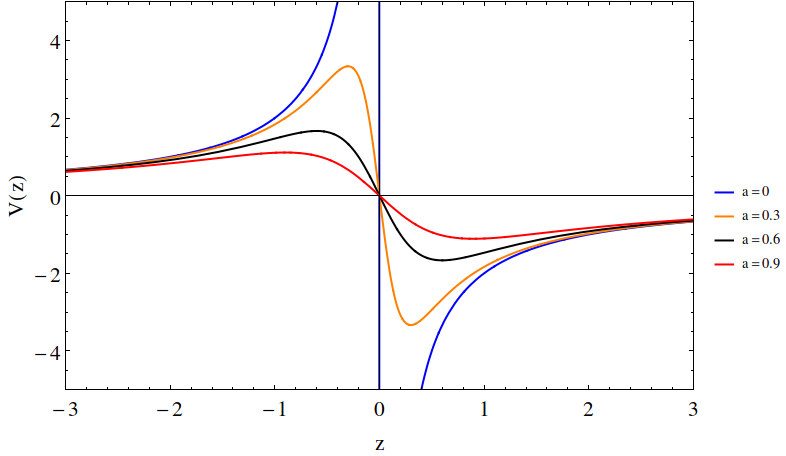
\includegraphics[width=\textwidth]{img/Chapter3/Potential.png}}
 \end{center}
 \caption{The potential $V(z)$ is displayed for various values of the parameter $a$. Note that the extremal points become lower as the parameter increases. For simplicity $M=1$ and $\lambda=1$ has been chosen. The potential for $\lambda=-1$ is the specular image of this representation using the $z$-axis as the axis of reflection.}
 \label{fig:Potentialeje}
\end{figure}  
\end{Remark}

\section{Variation ranges and causal structure}\label{causalstruct}
Since we are interested in causal and 
future
directed geodesics we need to find the restrictions on the initial data which 
guarantee this.
The following Proposition summarizes the results above and addresses the issue 
of future
directed initial data for both choices of $\sigma$.

Before we can start to study the variation ranges, we are going to define a new coordinate in which the metric does not depend if the spacetime is $(\mathcal{M},g|_{\lambda=1})=(\mathcal{Z}_1,g|_{\lambda=2})$ or  $(\mathcal{M},g_1)=(\mathcal{Z}_2,g_2)$. Defining 
\begin{equation}
 \bar{z}=\lambda z
\end{equation}
the metrics $g|_{\lambda=1}$ and $g|_{\lambda=2}$ become
 \begin{equation}\label{eq:KSmetricaxisnolam}
 ds^2=\eta + \lambda h K \otimes K =-dt^2+d{\bar z}^2+ \frac{2 M \bar z}{a^2+{\bar z}^2} (-\sigma dt + d \bar z) \otimes  (-\sigma dt + d \bar z)
\end{equation}
The equations of the \cref{Hamiltonianequivalence} become
 \begin{equation}
 E= \left (  1 -  h  \right ) \frac{d t}{ds}
+ h \sigma \frac{d {\bar z}}{ds},
 \end{equation}
 and the Hamiltonian is transformed to
 \begin{equation}
  \hat{H}=\frac{1}{2} \hat{p}_{\bar z}^2 -\frac{  \mu  M {\bar z}}{a^2+{\bar z}^2}
 \end{equation}
This can be done because the manifolds $\mathcal{Z}_1$ and $Z_2$ are diffeomorphic under the transformation $z \to -z$. By the use of this result, we can analyze more easily the variation ranges which are described in the following proposition.

\begin{proposition}\label{geodesicequationslema}
If the time orientation of $(\M,g)$ is chosen so that
the null vector 
$\partial_t +  \sigma  \partial_{{\bar z}}$
is future directed, then a geodesic with $\mu=0,1$ 
starting at a point $(t_0,{\bar z}_0)$ is future causal 
if and only if $\dot{{\bar z}}_0$ satisfies (with 
 $h_0 := h(|{\bar z}_0|)$)
 \begin{align*}
& \mbox{if }  h_0>1, \quad
\begin{cases}
\begin{aligned}
& \sigma \dot{{\bar z}}_0 \in [a_0, \infty) \\
&E = \pm \sqrt{\dot{{\bar z}}_0^2 - a_0^2 }
\end{aligned}
\end{cases}
\hspace{0.5cm}
\mbox{if }  h_0<1,  \quad
\begin{cases}
 \begin{aligned}
&  \sigma E \in [a_0, \infty) \\
&\dot{{\bar z}}_0 = \pm \sqrt{E^2 - a_0^2} \\
\end{aligned}
\end{cases}
\\
& \mbox{if }  h_0=1,  \quad  
\begin{cases}  
\begin{aligned}
& \sigma \dot{{\bar z}}_0 \in [0, \infty)  \quad \quad \mbox{with} \quad
\dot{{\bar z}}_0 =0 \Longrightarrow
\mu  =0 \\
&E =  \sigma \dot{{\bar z}}_0
\end{aligned}
\end{cases}
\end{align*}
where $a_0 ({\bar z}_0,\mu) := \sqrt{\left | 1-  h({\bar z}_0) \right | \mu } \geq 0$.
\end{proposition}
\begin{Proof}
 For the statements on the initial data, 
let $( t_0, {\bar z}_0 \neq 0)$ be the initial point of the geodesic
and $u_0 = (\dot{t}_0, \dot{{\bar z}}_0)$ the initial velocity, 
normalized to satisfy $g(u_0,u_0) = -\mu$ ($\mu = 0,1$) and assumed
to be future directed. 
Recall that the Kerr-Schild vector is $K^{\alpha} = (\sigma, 
)$. the choice of time orientation means
that $\sigma K^{\alpha}$ is future directed. thus,
$u_0$ being future directed is equivalent to 
$g(u_0, \sigma K |_{s=0}) <0$ or $u_0 = b \sigma K|_{s=0}$, with $b \geq 0$. 
to compute $g(u_0, \sigma K|_{s=0})$ observe that $g(\sigma K, \cdot ) =
 -  dt +  \sigma d {\bar z}$ which implies
\begin{equation}
\label{product}
g(u_0, \sigma K|_{s=0} ) =  \sigma \dot{{\bar z}}_0 - \dot{t}_0 .
\end{equation}
On the other hand, the condition $u= b \sigma K|_{s=0}$ ($b \geq 0$)
is ($\dot{t}_0 = b, \dot{{\bar z}}_0 = b \sigma $)
or equivalently $(\dot{t}_0 = \sigma  \dot{{\bar z}}_0  \geq 0)$. 
the \cref{eq:conservedenergy,ener} evaluated at $s=0$ read
\begin{align}
& E^2 = \dot{{\bar z}}^2_0 + \mbox{sign}(1- h_0) a_0^2, \label{energy2} \\
& E  = \left ( 1-  h_0  \right ) \dot{t}_0 + h_0  \sigma \dot{{\bar z}}_0, \label{E2}
\end{align}
where $\mbox{sign} (1- h_0)$ takes the values $1,0,-1$ depending
on whether $ h_0 < 1$, $ h_0=1$ or $ h_0>1$ respectively
and $a_0$ is as defined in the statement of the theorem.
At points $ h_0 \neq 1$, \cref{energy2,E2} imply $g(u_0,u_0) = -\mu$.
However, when $ h_0=1$, 
\cref{energy2} is a trivial consequence
of \cref{E2} and $g(u_0,u_0)= - \mu$ must be imposed 
additionally. We compute (with $ h_0=1$)
\begin{align}
-\mu & = g (u_0,u_0) = \eta(u_0,u_0) + h_0 \left ( \bm{K} |_{s=0} (u_0) \right 
)^2 =\nonumber\\\
&= - \dot{t}_0^2 + \dot{{\bar z}}_0^2 + g(\sigma K|_{s=0},u_0)^2 = \nonumber \\
& = 2 \sigma \dot{{\bar z}}_0 \left ( \sigma \dot{{\bar z}}_0 -  \dot{t}_0 \right ) ,
\label{caseh0=1}
\end{align}
where (\ref{product}) has been used in the last equality.

We can now find the most general $u_0$ satisfying all these
restrictions. the analysis depends on whether $ h_0>1$ $ h_0 <1$ 
or $ h_0=1$. We start with $ h_0 \neq  1$.
Because of (\ref{E2}),
the initial data $\dot{t}_0$  can be substituted by the value of $E$.
Moreover,
\begin{align*}
(1 -  h_0)^2 g(u_0, \sigma K|_{s=0}) &= (1-  h_0 ) \left ( ( +  h_0-1  ) \dot{t}_0
+ (1-   h_0) \sigma  \dot{{\bar z}}_0 \right ) \\
&= \left ( h_0 -1 \right ) \left ( E - \sigma \dot{{\bar z}}_0 \right ),
\end{align*}
where (\ref{E2})
has been again inserted in the last equality. 
thus, the statement $g(u_0, \sigma K_0|_{s=0}) < 0$  or 
$u_0 = b \sigma K|_{s=0}$ with $b \geq 0$ is equivalent to
\begin{gather*}
(h_0 -1 ) (E -  \sigma \dot{{\bar z}}_0 ) < 0 \quad \mbox{ or } \quad 
 E = \sigma  \dot{{\bar z}}_0 \geq  0,
\end{gather*}
the second inequality being a consequence of $\dot{t}_0 =  \sigma \dot{{\bar z}}_0 \geq 0$ and (\ref{E2}). Assume now $ h_0 >1$. the conditions to be imposed are 
$\{ E <  \sigma \dot{{\bar z}}_0$ or $E =  \sigma \dot{{\bar z}}_0  \geq 0\}$,
together with $E^2 = \dot{{\bar z}}_0^2 - a_0^2$ 
(from equation (\ref{energy2})). the locus of this quadratic equation is a hyperbola 
with two branches (degenerating to two straight lines when $a_0=0$)
and with asymptotes $E = \pm \dot{{\bar z}}_0$. the condition
$\{ E <  \sigma \dot{{\bar z}}_0$ or $E =  \sigma \dot{{\bar z}}_0 \geq 0\} $ selects
precisely the branch satisfying 
$ \sigma \dot{{\bar z}}_0 \geq  a_0$, as claimed in the Proposition.
the case $ h_0 <1$ is analogous:  the conditions are now
$\{ E >  \sigma \dot{{\bar z}}_0$ or $E =  \sigma \dot{{\bar z}}_0 \geq 0\}$ together
with
$E^2 = \dot{{\bar z}}_0^2 + a_0^2$. the solution to these inequalities
is the branch of the hyperbola satisfying 
$\sigma E \geq a_0$.

For the case $ h_0=1$, equation (\ref{caseh0=1}) reads
\begin{equation}
2 \sigma \dot{{\bar z}}_0 \left( \sigma \dot{{\bar z}}_0 -  \dot{t}_0
\right) = -  \mu  \leq 0.
\label{caseh1}
\end{equation}
thus, the condition
$\{ \sigma \dot{{\bar z}}_0 -  \dot{t}_0 < 0$ or $\dot{t}_0 =  \sigma \dot{{\bar z}}_0 \geq  0\}$
is equivalent to $ \sigma \dot{{\bar z}}_0 \geq 0$ and zero only if
$\mu = 0$. this is because, when $ \sigma \dot{{\bar z}}_0 >0$,  
equation (\ref{caseh1}) can be solved uniquely for $\dot{t}_0$ 
with the solution satisfying $\sigma \dot{{\bar z}}_0 -  \dot{t}_0 \leq 0$,
that is, either $\sigma \dot{{\bar z}}_0 -  \dot{t}_0 < 0$ or 
$\dot{t_0} =  \sigma \dot{{\bar z}}_0 > 0$.
When $\sigma  \dot{{\bar z}}_0 =0$ then $\mu=0$ and
$ \dot{t}_0 \geq 0$ is arbitrary, so again
we satisfy  $\{ \sigma \dot{{\bar z}}_0 -  \dot{t}_0 <0$ 
or $\dot{t}_0 =  \sigma \dot{{\bar z}}_0 \geq 0\} $. 
Finally, the statement $E=  \sigma \dot{{\bar z}}_0$ when $h_0=1$ 
follows directly from (\ref{E2}).
\end{Proof}

\begin{Remark}
Note that when $\mu=0$ we have $a_0 \equiv 0$
and this Proposition admits the initial data 
$\dot{r}_0 =0, E=0$ irrespectively
of the value of $h_0$. When $h_0\neq 1$, this boundary case corresponds to the
situation when the initial tangent four-vector 
vanishes, and hence the geodesic is a trivial curve. This is consistent
with the fact that the zero vector is null and future directed.
Admitting trivial curves as null future directed geodesics
has the advantage that allows one to treat at once the cases $\mu =0$ and
$\mu =1 $. 
\end{Remark}

\begin{corollary}\label{epsilonrange}
The variation ranges for $\epsilon$ are
\begin{equation}
\begin{cases}
\epsilon \in [-\frac{\mu}{2},\infty) &\mbox{if } h_0 \geq 1\\
\epsilon \in [\frac{a_0^2-\mu}{2},\infty) &\mbox{if } h_0<1
\end{cases}
\end{equation}
independently of the sign of $\sigma$  and of the function $h(\vec{x})$ in the 
Kerr-Schild metric.
\end{corollary}
\begin{Proof} Immediate from the ranges of variation of $E$
in Proposition \ref{geodesicequationslema} 
and the relation $\epsilon=\frac{1}{2} (E^2-\mu)$.
\end{Proof}

This information will be very useful because this will allow us to distinguish and categorize the different curves that will appear in the phase space of the spatial part of the geodesic movement. In the future phase space we will deal with curves that cross multiple time the different horizons and that are traveling through the \gls{PC} diagram of the $z$-axis of the Kerr spacetime that is displayed in \cref{fig:Penrose2}, changing from $\gls{KS}$ patch over and over.

 \begin{figure}[htp!]
\begin{center}
 \centerline{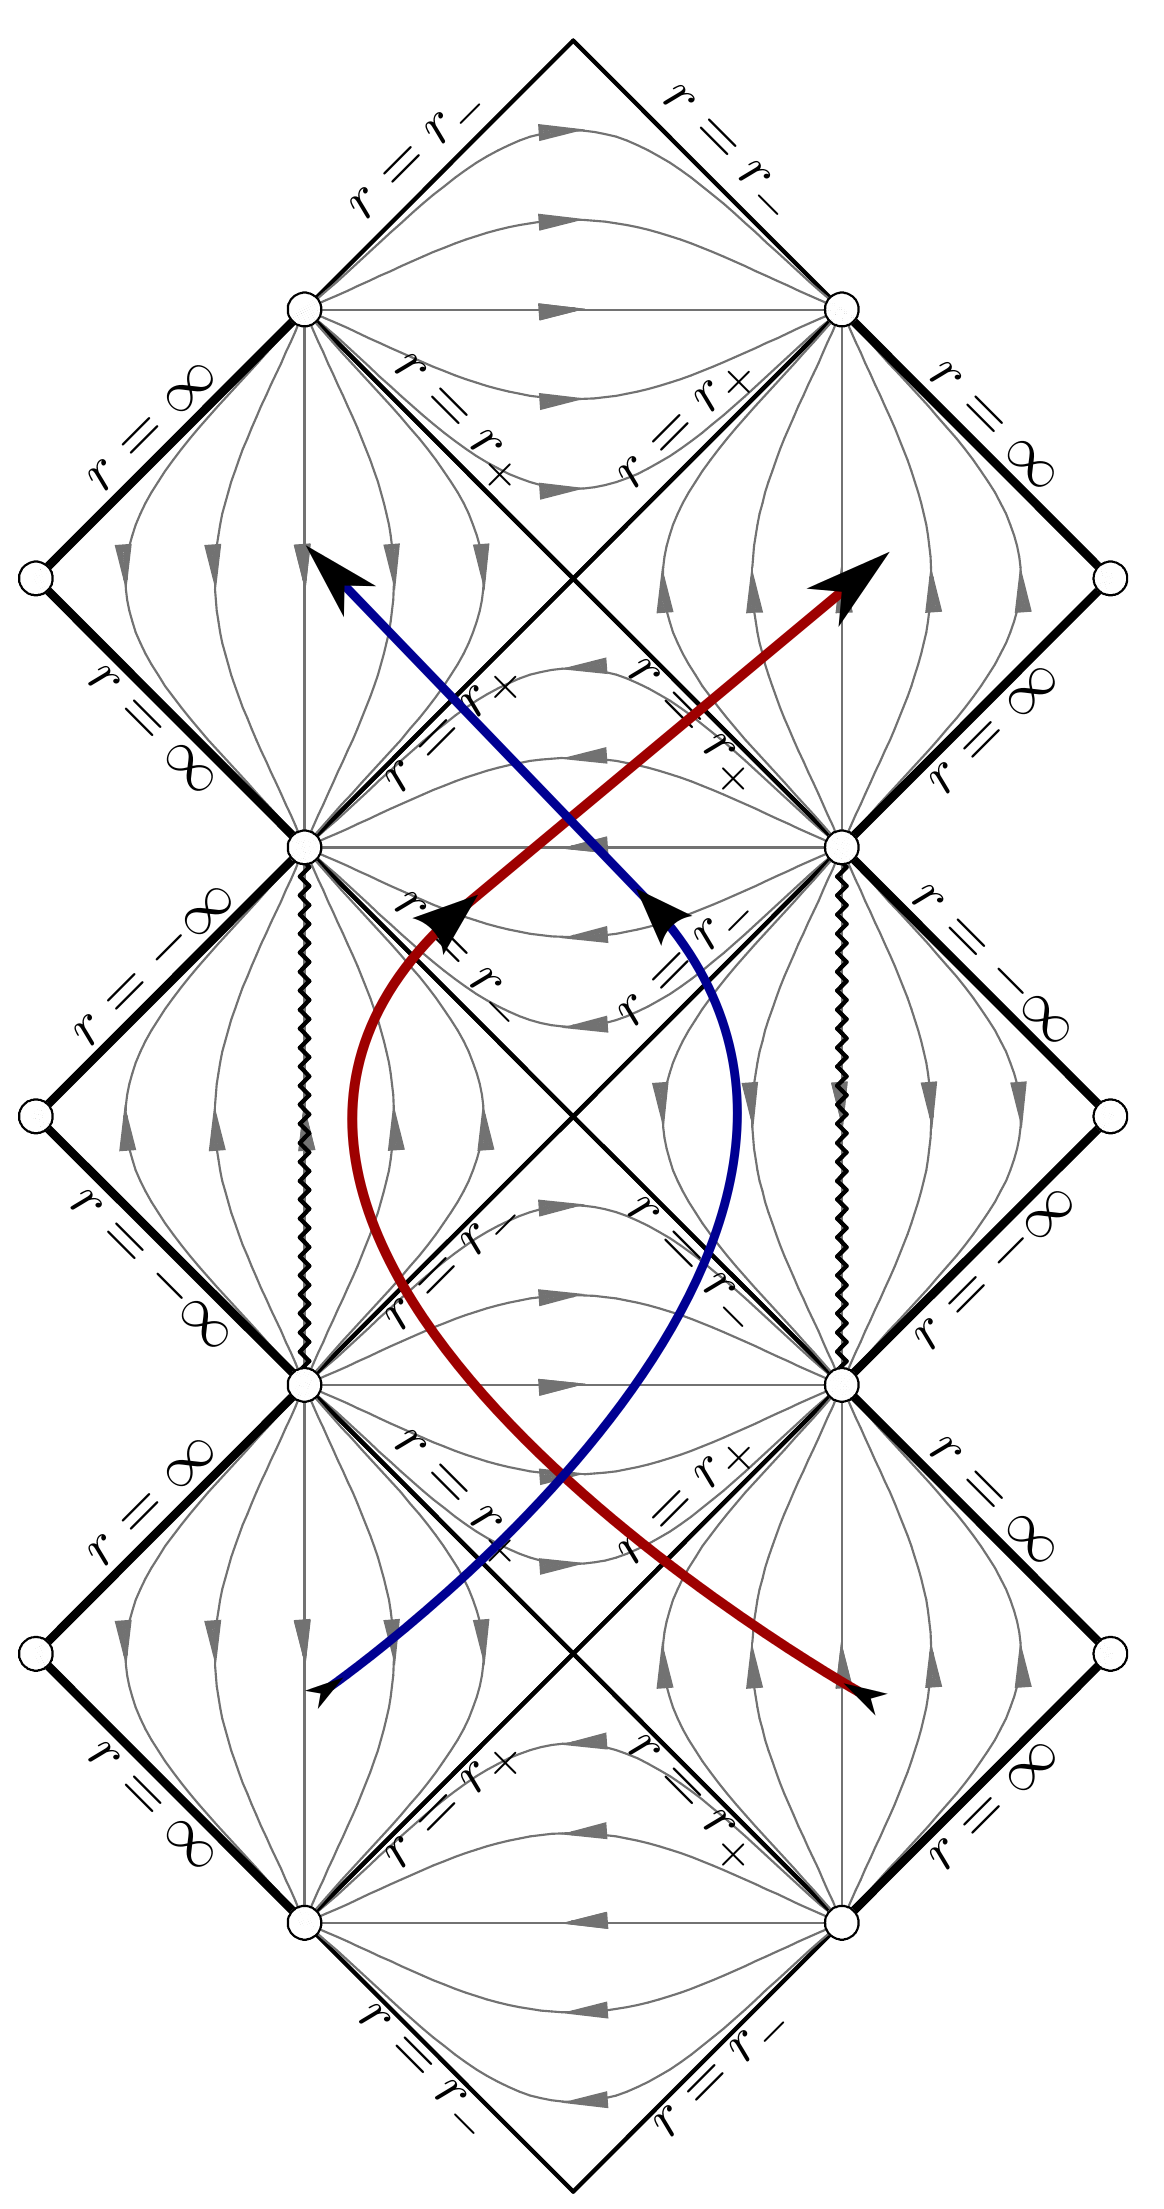
\includegraphics[width=.38\textwidth]{img/Chapter3/Diagrama2.png}}
 \end{center}
 \caption{\gls{PC} diagram of the Kerr spacetime along the axis of symmetry for simplicity. The red path represents a geodesic that crosses $r=r_+$ twice and changes from the \gls{KS} patch in which $\sigma=1$ to the patch in which $\sigma=-1$. The blue curve is analogous to the red one but for a geodesic that starts in the isometric region of the left. This isometric regions are disconnected as are remarked in the text. Remember that for the $z$-axis the coordinate $r=\lambda z= \bar z$.}
 \label{fig:Penrose2}
\end{figure} 
\FloatBarrier

By the use of the \cref{geodesicequationslema} we can know that a geodesic that start in the \gls{KS} patch with $\sigma=1$ (see \vref{fig:PenroseKS} to see the \gls{KS} patches ) that crosses the even horizon at $\bar z=r_+$ for the first time, cannot cross the same even horizon at $\bar z=r_+$ (in the same \gls{KS} patch) because once crossed this point with $\sigma=-1$ then $\dot{r}=\dot{ \bar z} <0$ and therefore as $-\infty < r_- <r_+ < \infty$ the geodesic cannot go back to the asymptotically flat region of the \gls{KS} patch where it stated. In the other hand the same geodesic can continue its journey through $\bar z=r_-$ and once crossed this point change to the \gls{KS} patch with $\sigma=+1$ and then cross $\bar z=r_-$ again (moving upwards in the \gls{PC} diagram of \cref{fig:Penrose2}). Once $\bar z=r_-$ is crossed in the patch with $\sigma=+1$ the variation ranges in this region imply $\dot{r}=\dot{\bar z} >0$ and therefore the geodesic cannot go back to $\bar z=r_-$ but it can cross the even horizon at $\bar z=r_+$ in the \gls{KS} patch with $\sigma=+1$ and continue to the asymptotically flat region of the \gls{KS} patch with $\sigma=+1$. This behavior can be summarized in the fact that if a geodesic cross twice $\bar z=r_+$ its traveling upwards in the \gls{PC} diagram and therefore changing from one \gls{KS} patch to another. This can be done as many times as needed and the geodesic journey can stop in any of the infinite asymptotically flat regions.

Notice that there is no
causal geodesic starting from a left-most quadrant 
which, after  crossing 
the null hypersurface $\bar z=r_+$ then
goes across the portion of the null hypersurface at $\bar z=r_-$ 
lying at the left of the diagram (and similarly for geodesics starting
at a  right-most quadrant). The
reason is that  the Killing 1-form 
$dt := g(\partial_t,\cdot)$ (defined on a single \gls{KS} patch) is integrable with
orthogonal hypersurfaces foliating the region $r_{-} < z < r_{+}$
with timelike leaves. Let us label these leaves by $T$. As a
consequence we have $dt = G d T$ on $r_{-} < z < r_{+}$
where $G$ is a smooth function.
Consider the 
conserved energy for the geodesic, i.e. $ \langle \partial_t, u \rangle =-E $
where $u$ is the tangent vector. In the region between
$r_-$ and $ r_+$, in order for the geodesic to enter from the left portion of
the null hypersurface $\bar z= r_{+}$ and leave across the left portion
of the hypersurface $\bar z=r_{-}$, the geodesic must become somewhere tangent
to a hypersurface $T= \mbox{const}$. At this point we have $-E = dt (u) =
G dT (u) = 0$.
But $E=0$ is impossible for a geodesic starting on the left-most region
where $\partial_t$ is timelike. A similar argument applies to geodesics
starting at the right-most quadrant.

\section{Phase space and dynamic equations}

Now that we know how to distinguish geodesics in the spacetime and we understand how the causal structure of the spacetime works and which kind of flows can be expected, we are ready to obtain the dynamic equations that describe the phase space of the spatial part of the geodesics in the axis of symmetry of the Kerr metric. From \cref{Hamiltonianequivalence} we have that the spatial part of the geodesic flow is carried by the Hamiltonian 
\begin{equation}
\hat{H}=T+V(z)=\frac{1}{2} \hat{p}_z^2 -\frac{ \lambda  \mu  M z}{a^2+z^2} .
\end{equation}
where $H=\epsilon=\frac{1}{2}(E^2-\mu)$. The Hamilton equations for this Hamiltonian are
\begin{align}
 z'(s)&= p_z  \label{Hamiltoneq1}\\
 p_z'(s)&=-\lambda (( M (-a^2 + z^2))/(a^2 + z^2)^2)\label{Hamiltoneq2}
\end{align}

\subsection{Null geodesics}

If we set $\mu=0$ (null geodesics), the dynamic equations of \cref{Hamiltoneq1,Hamiltoneq2} take the form
\begin{align}
 z'(s)&= p_z  \\
 p_z'(s)&=0
\end{align}
and therefore the solution of the system is
\begin{align}
 z(s)&=z_0 +{p_z}_0 s \\
 p_z(s)&={p_z}_0
\end{align}
where $z(0)=z_0$ and $p_z(0)={p_z}_0$. Hence, the null geodesic along the symmetry axis of the Kerr spacetime move with constant velocity unaffected by any gravitational force. This is quite interesting because this geodesics can travel through the inner disk ($z=0$) and go from one copy of $\mathbb{R}_\pm$ to another at constant velocity ${p_z}_0$. For the null geodesics there is no fixed points and no excluded regions. In the phase portrait of \cref{fig:photons} it can be appreciated that for $p_z=z'>0$ all geodesics are in the \gls{KS} patch with $\sigma=1$ because between the horizons $r_-< \lambda z < r_+$ only particles with $z'>0$ are allowed and for $p_z=z'<0$ all geodesics are in the \gls{KS} patch with $\sigma=-1$ because between the horizons $r_-< \lambda z < r_+$ only particles with $z'>0$ are allowed.

 \begin{figure}[hpt!]  
\begin{center}
 \centerline{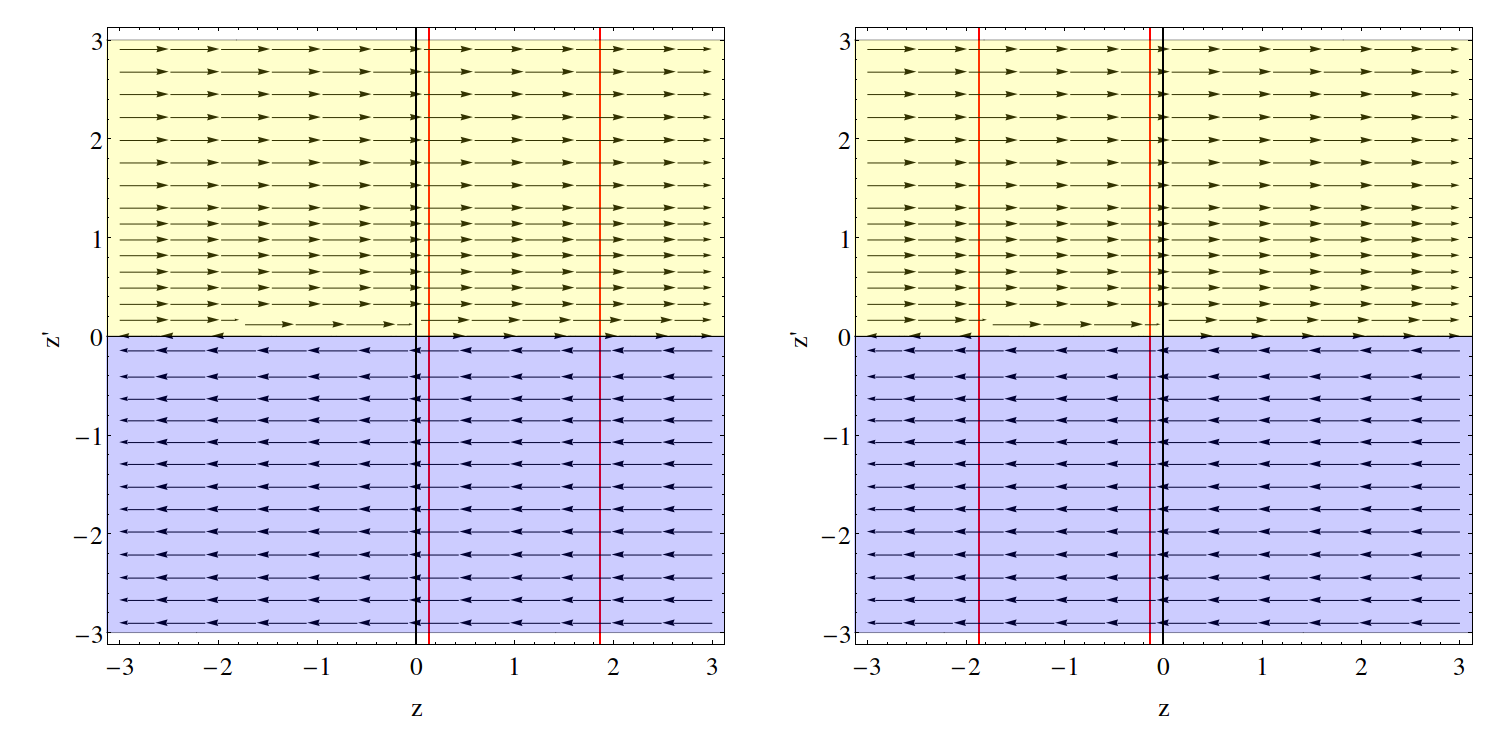
\includegraphics[width=\textwidth]{img/Chapter3/photonsps.png}}
 \end{center}
 \caption{Phase portraits for the null geodesic in the axes of symmetry. The picture on the left shows the phase space for $\mathcal{Z}_1$ while the picture on the right shows the phase space for  $\mathcal{Z}_2$. The black thick lines represent the axis ($\{z=0,z'=0\}$), the red thick lines represent the horizons at $r=r_\pm$ (notice that $0<r_-<r_+$ for $\mathcal{Z}_1$ as $r=z$ and $0>r_->r_+>$ for $\mathcal{Z}_2$ as $r=-z$). The yellow region indicates the region with $\sigma=1$ and the blue region indicates the region with $\sigma=-1$}
 \label{fig:photons}
\end{figure}  


\subsection{Timelike geodesics}

Despite the behavior for null geodesics is quite simple, the behavior for timelike geodesics is not simple at all. In fact,  there are now excluded regions provided by \cref{epsilonrange} that cannot be accessible to the flow of the timelike geodesics in the phase space. The shape of this excluded regions change with the value of the parameter $a$ (as the Kerr black hole spins faster) and must be studied independently to fully understand the dynamic system and the phase portrait that will be displayed along the analysis of the timelike geodesics.
\FloatBarrier
\subsubsection{Excluded regions}\label{excludedreg}
 \begin{figure}[htp!]
\begin{center}
 \centerline{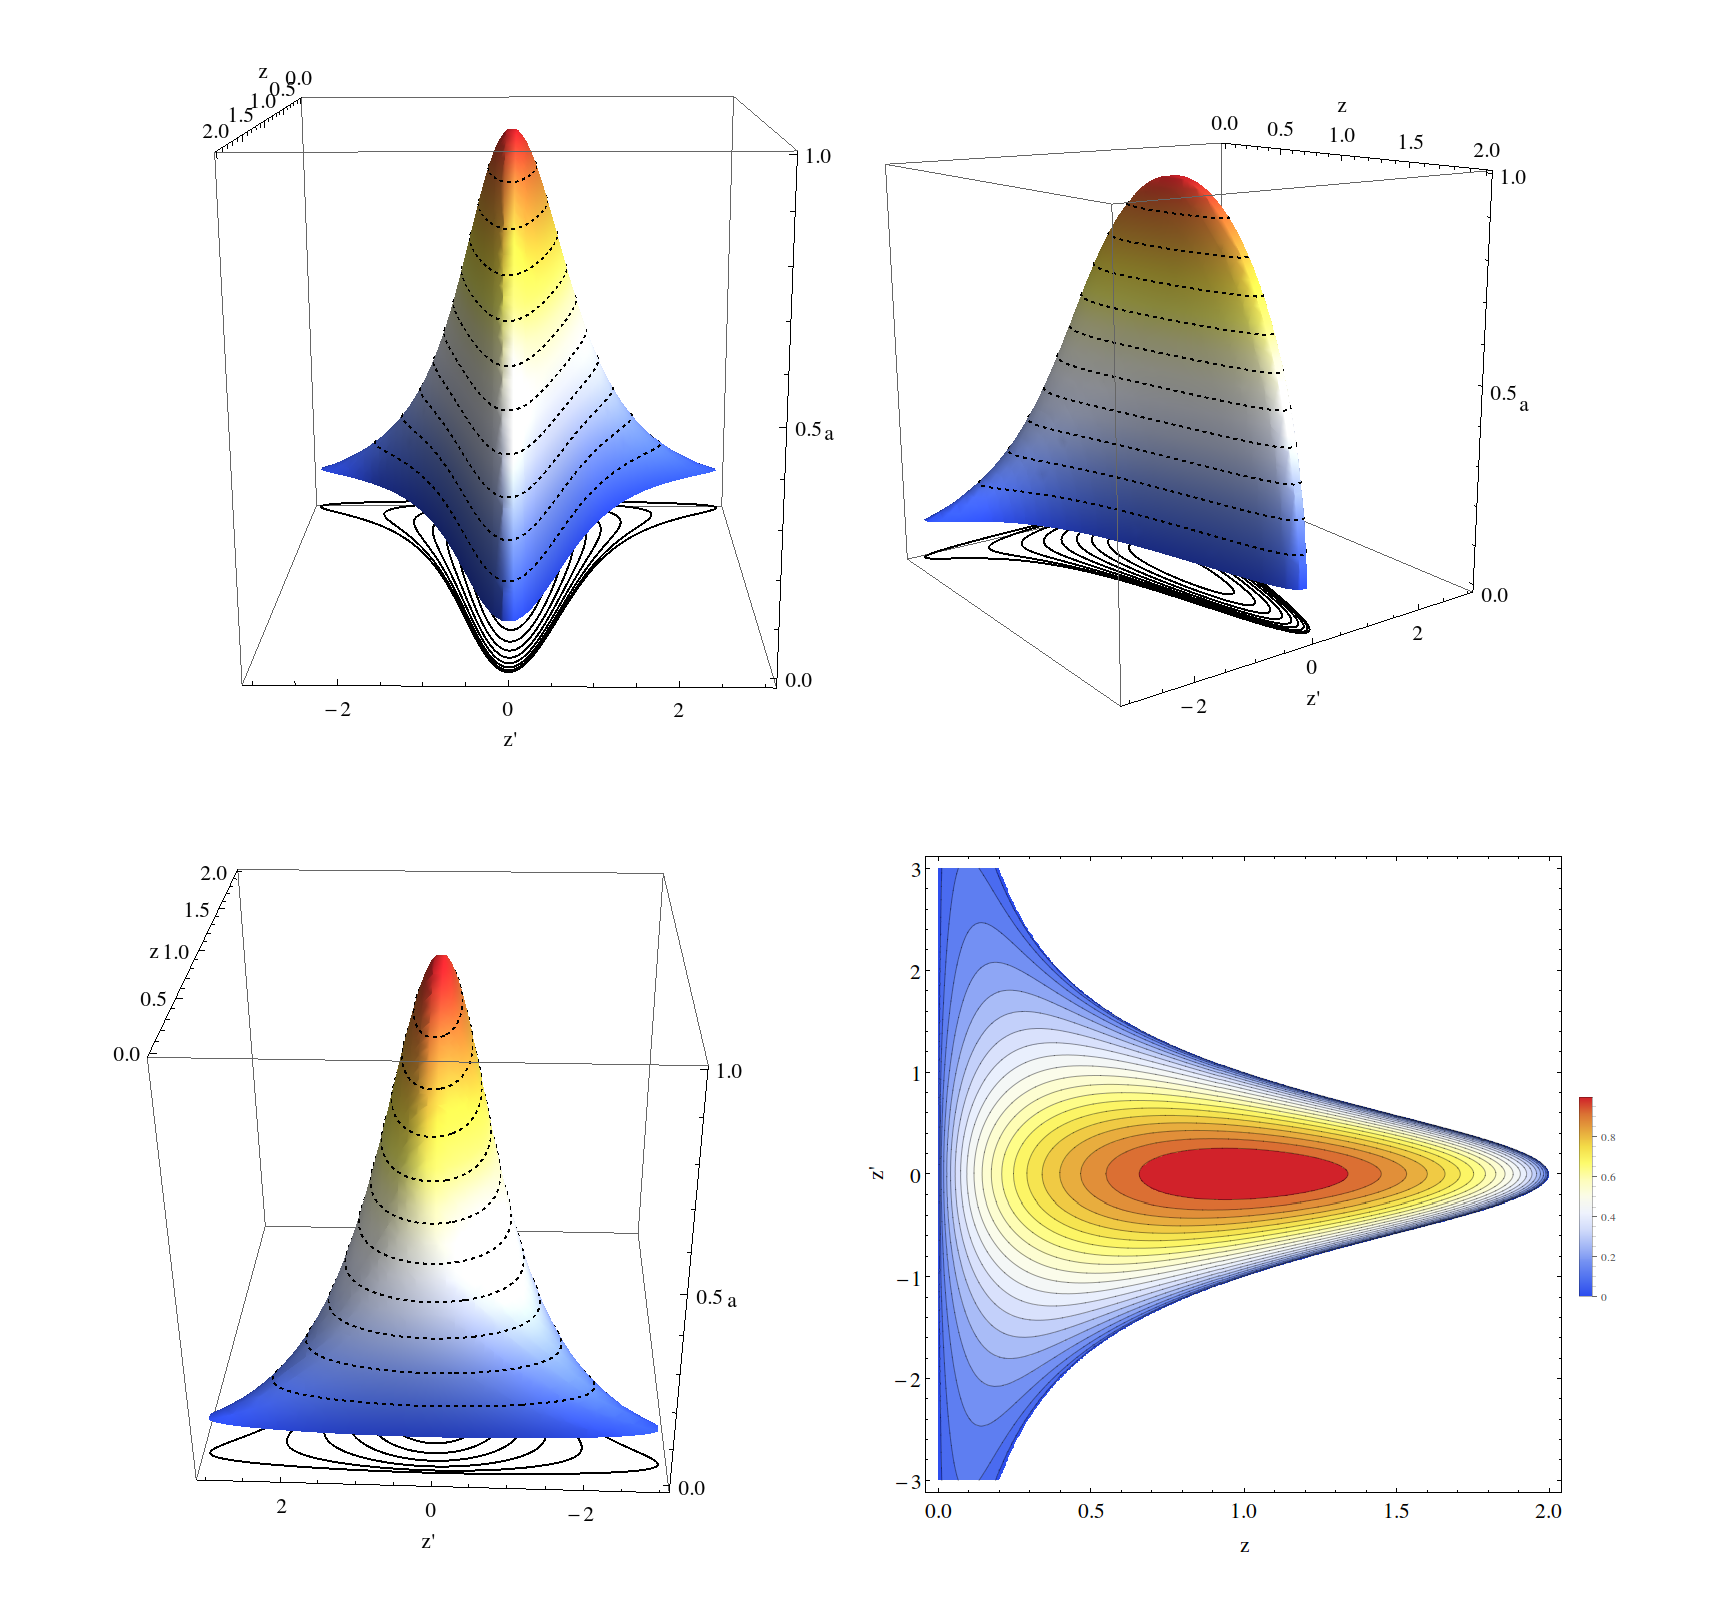
\includegraphics[width=\textwidth]{img/Chapter3/Excluded.png}}
 \end{center}
 \caption{Excluded regions for timelike geodesics and their their dependence with the value of the parameter $a$. The vertical axis represents the value of $a$ (as also the coloring). The other axes represent the values of $z$ and $z'$. The bottom right picture shows the projection onto the $\{z,z'\}$ plane, which is the phase portrait (the colors serve to help the visualization of the variation with the parameter $a$). As we can see in the images, the ''area'' of the excluded regions decreases when the parameter $a$ increases and the excluded region vanishes for $a=M$. Also, the excluded regions move across the $\{z,z'\}$ plane as the parameter $a$ increases. For simplicity $M=1$ and $\lambda=1$ is chosen.}
 \label{fig:Excluded}
\end{figure} 
As was noticed before, the allowed variation range is traduced into the existence of excluded regions in the phase space. The existence of this excluded regions is very important because provided the necessary topology to the phase space in order to describe all the geodesic flow for timelike particles in the \gls{MAE} of the symmetry axis of the Kerr spacetime. If the phase space would have trivial homotopy class it could be impossible to ``project'' the geodesic flow across the \gls{MAE} of the symmetry axis of the Kerr spacetime in one bi-dimensional space phase because all the trajectories that cross the horizons and change between the infinite \gls{KS} patches could not be displayed.

By the use of \cref{epsilonrange} we find that the expression for the excluded regions of timelike particles are written as
\begin{equation}
\frac{1}{2} \hat{p}_z^2 -\frac{ \lambda M z}{a^2+z^2}<\frac{1}{2}
\end{equation}
As we see in \cref{fig:Excluded} the excluded regions are like ''bubbles'' that decreases size when $a \to M$, vanishing when $a=M$ (extreme Kerr spacetime). Also, the ''bubbles`` are Are attached to the axis $z = 0$ for $a=0$ and they detach from this axis while $0<a<M$ as they travel along the phase space. The excluded regions are always limited for the horizons at $\bar z= r_\pm$, as the origin of this excluded regions are the limitations into the initial parameters that the time orientation provides. Also, because in $\mathbb{R}_-$ there is no horizons, there are not excluded regions in this region of $\mathcal{Z}_1$ and $\mathcal{Z}_2$, which corresponds to $z<0$ in $\mathcal{Z}_1$ and $z>0$ in $\mathcal{Z}_2$. The boundary of the excluded regions belongs to the phase space because the limit case $\frac{1}{2} \hat{p}_z^2 -\frac{ \lambda M z}{a^2+z^2}=\frac{1}{2}$ is a physical trajectory for the geodesic motion and is included in the phase space. Notice also that \cref{geodesicequationslema} excludes the possibility of having a geodesic in the point $\bar z=a$ the case where $a=M$ (in which there are no excluded regions and the horizons collapse in one unique surface at $\bar z=a$) because this is only allowed for null geodesics $\mu=0$. The reason is that for $a=M$ the horizons are at $\bar z=0$ and because this surfaces are null hypersurfaces, only null tangent vectors can move remain in them, and therefore, timelike particles are not allowed to remain in this point (unless as we will see it is a stable point) despite there are no apparent excluded regions.
 
 
\subsubsection{Phase space}

If we set $\mu=1$ (timelike geodesics), the dynamic equations of \cref{Hamiltoneq1,Hamiltoneq2} take the form
\begin{align}
 z'(s)&= p_z , \\
 p_z'(s)&=-\lambda \frac{M \left(z^2-a^2\right)}{\left(a^2+z^2\right)^2}.
\end{align}
Remember that because the Hamiltonian itself is a first integral with value $\epsilon=\frac{1}{2}(E^2-1)=\frac{1}{2} \hat{p}_z^2 -\frac{ \lambda  \mu  M z}{a^2+z^2}$. The dynamic system for timelike geodesic present very interesting features that can be observed in \cref{fig:Phasediagrams}. The fixed points of the system are given by the equations
\begin{align}
  z'(s)&= 0 \quad \Longrightarrow \quad p_z=0,\\
  p_z'(s)&=0 \quad \Longrightarrow \quad -\lambda \frac{M \left(z^2-a^2\right)}{\left(a^2+z^2\right)^2}=0.
\end{align}
  \begin{figure}[htp!]  
\begin{center}
 \centerline{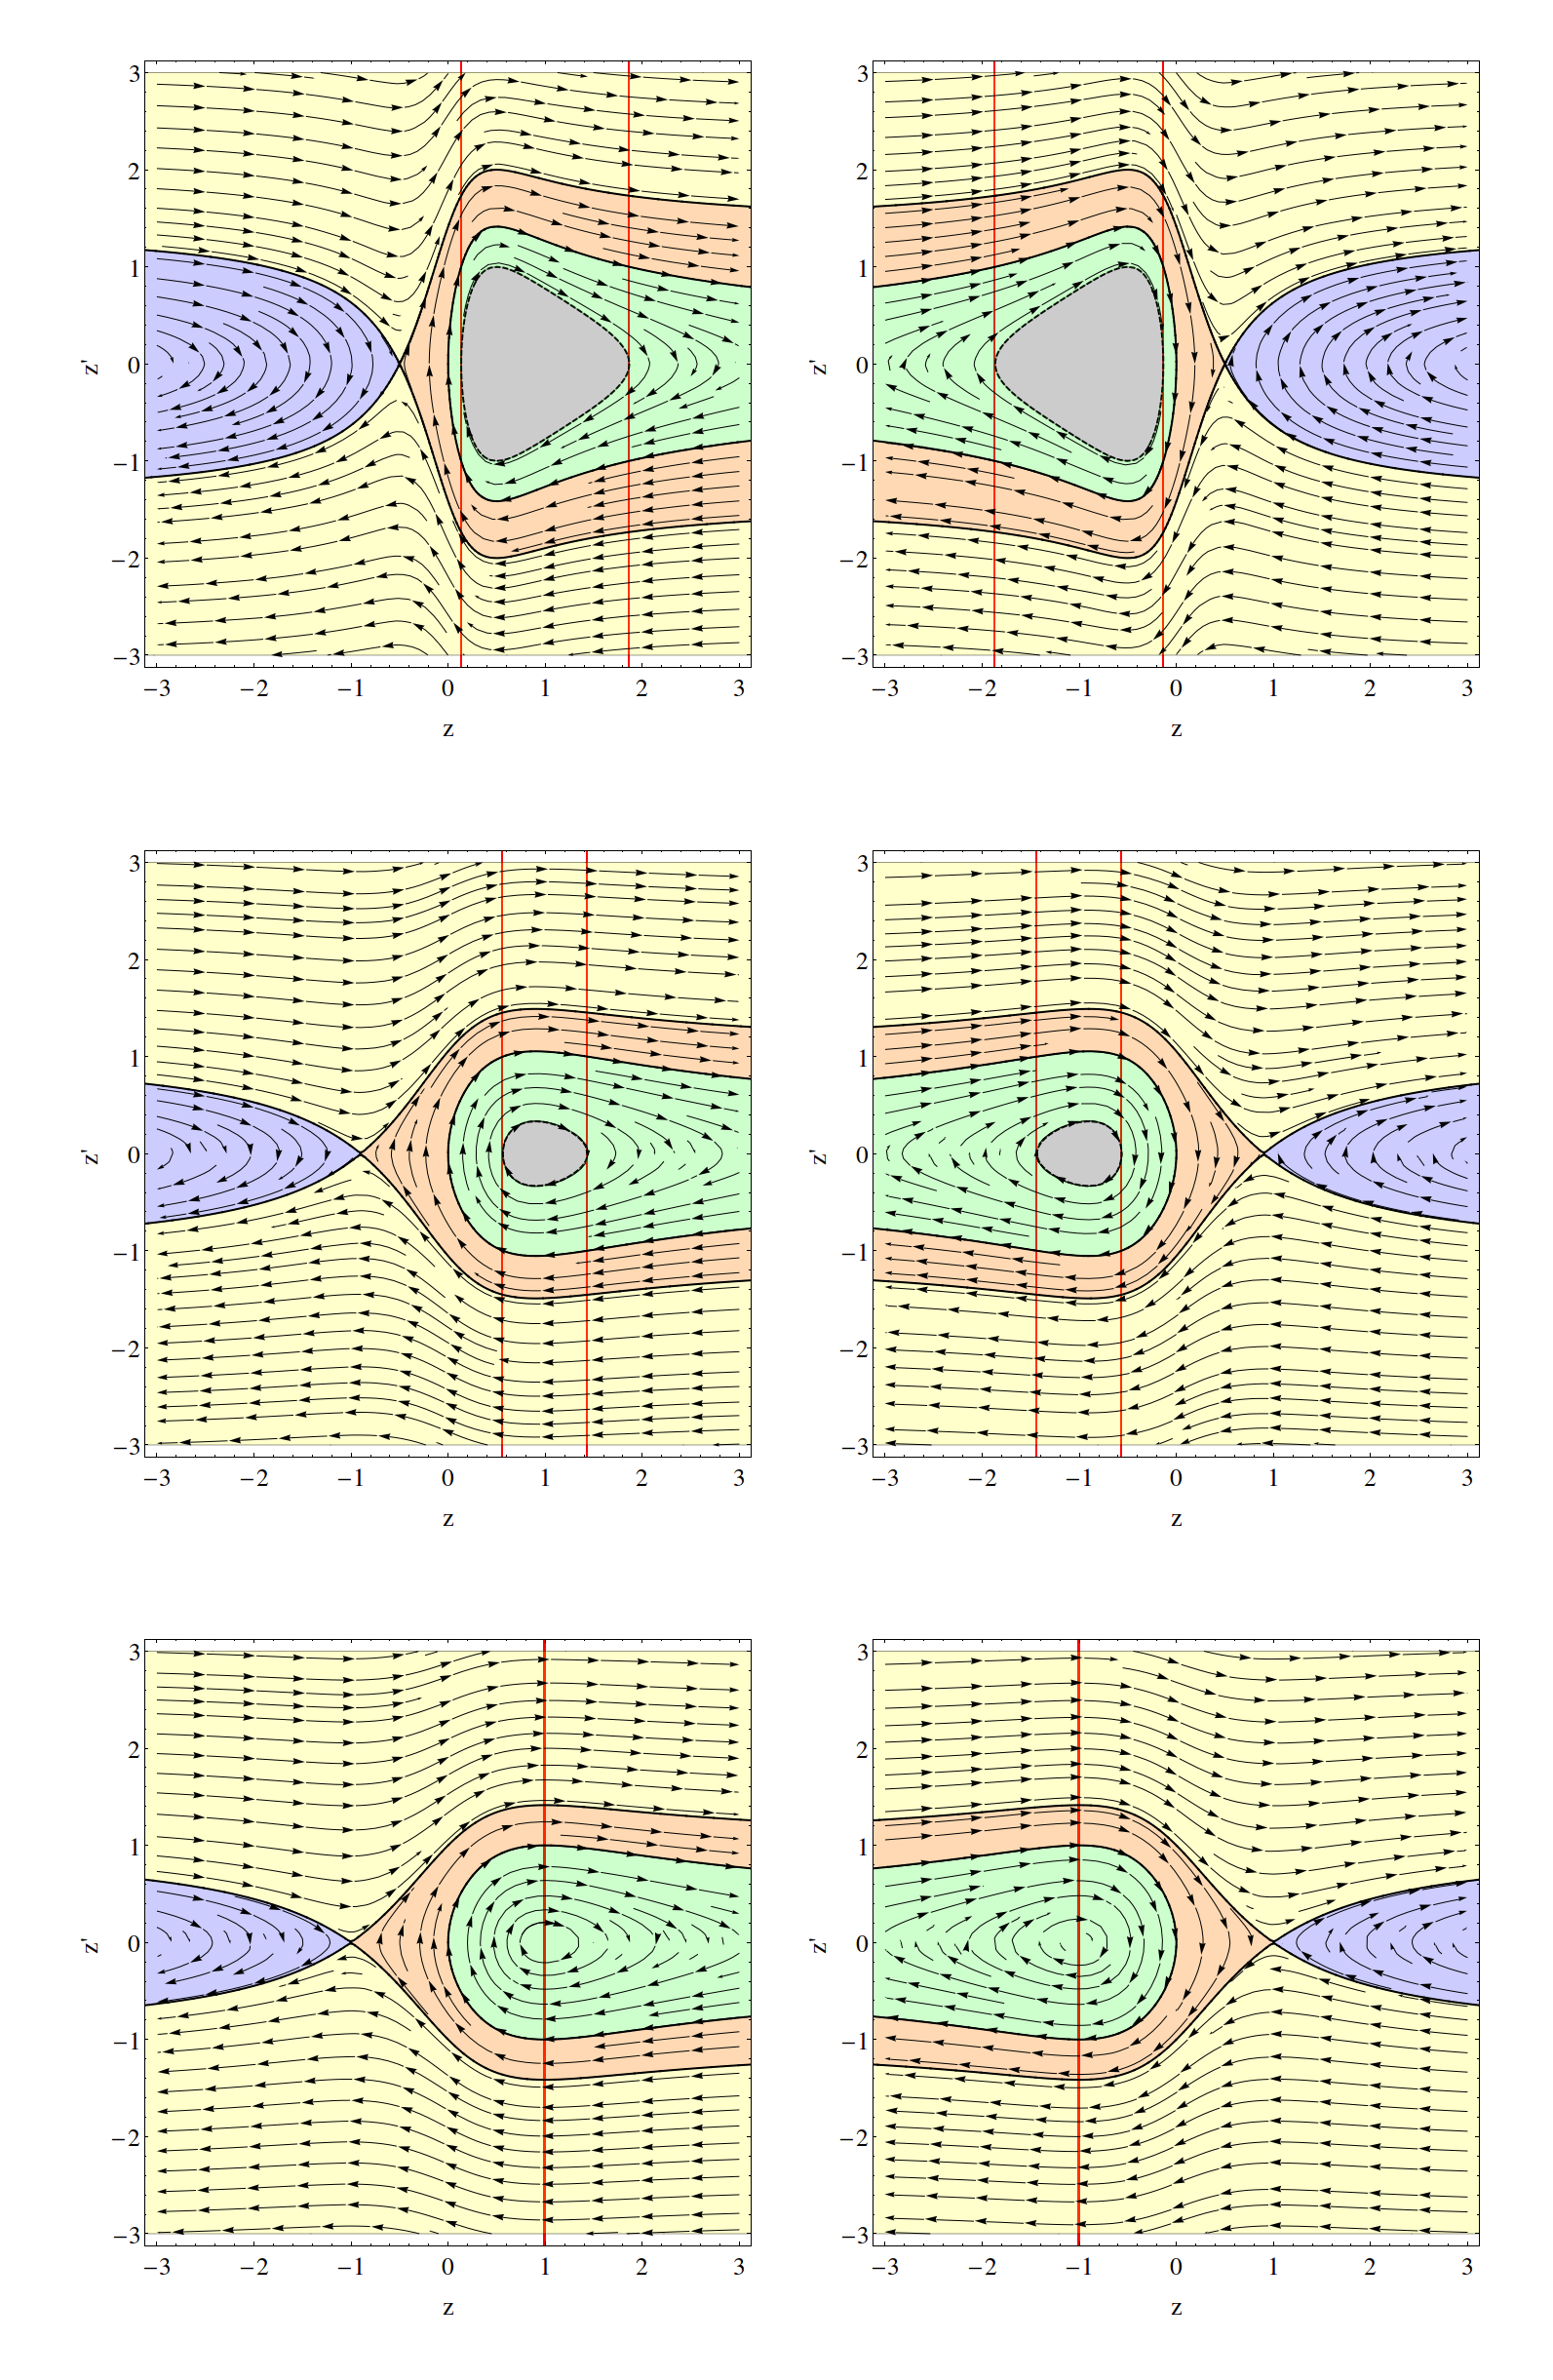
\includegraphics[width=0.95\textwidth]{img/Chapter3/Phase.png}}
 \end{center}
 \vspace{-1.5cm}
 \caption{The phase spaces for timelike geodesic are displayed. The left column shows to the phase space for $\mathcal{Z}_1$ and the right column for $\mathcal{Z}_2$. In each column the phase portraits for the values $a=\{0.8 M,0.9 M,M\}$ are displayed (top to bottom). The red lines corresponds to the horizons at $\bar z=r_\pm$. The red region corresponds to the excluded region, the yellow region represent the curves in the phase space that connects $\bar z= \infty$ with $\bar z= -\infty$, the blue area represent the curves that start in $\bar z=-\infty$ and return to $\bar z=-\infty$, the orange zones represent the curves that start in $\bar z=\infty$ and end in $\bar z=\infty$. The closed curves are in the green area and the limit orbit is the black dashed line surrounding the excluded region. $M=1$ is settled for simplicity.}
 \label{fig:Phasediagrams}
\end{figure}  
The solution of this system is
\begin{equation}
 z_\pm= \pm a \quad \mbox{and} \quad p_z=0
\end{equation}
The nature of the fixed points is obtained linearising the system around them. The linealization is given by
\begin{equation}
\left(
\begin{array}{c}
 \delta z'(s) \\
 \delta p_z'(s)
\end{array}
\right)= J|_{z=z_\pm,p_z=0} \left(
\begin{array}{c}
 \delta z(s) \\
 \delta p_z(s)
\end{array}
\right).
\end{equation}
where the Jacobian matrix ($J$) is given by
\begin{equation}
J=\left(
\begin{array}{cc}
 \frac{\partial z'(z,p_z)}{\partial z} & \frac{\partial z'(z,p_z)}{\partial p_z} \\
 \frac{\partial p_z'(z,p_z)}{\partial z} & \frac{\partial p_z'(z,p_z)}{\partial p_z}
\end{array}
\right)=\left(
\begin{array}{cc}
 0 & 1 \\
 -\frac{M \gamma \lambda }{2 a^3} & 0 \\
\end{array}
\right),
\end{equation}
where the sign $\gamma=\pm 1$ corresponds to $ z= \gamma a$. The eigenvalues of the Jacobian matrix are
\begin{align}
 \lambda_1&=-\frac{\sqrt{-\lambda \gamma M }}{\sqrt{2a^3 }},\\
 \lambda_2&=\frac{\sqrt{-\lambda \gamma M }}{\sqrt{2 a^3} }.
\end{align}
The eigenvalues are real iff $\lambda \gamma = -1$, which corresponds to $z=-a$ in $\mathcal{Z}_1$ and $z=a$ in $\mathcal{Z}_2$. When the eigenvalues are real, they have also opposite signs, and therefore $z=-a$ in $\mathcal{Z}_1$ and $z=a$ in $\mathcal{Z}_2$ are unstable saddle points. When $\lambda \gamma = +1$ the eigenvalues are purely imaginary and corresponds to $z=a$ in $\mathcal{Z}_1$ and $z=-a$ in $\mathcal{Z}_2$. As the eigenvalues in this case are complex conjugate they corresponds to a stable point that happens to be a center. Notice that this eigenvalues are always inside the excluded region and therefore no timelike geodesic can rest in the stable center point. The only movement allowed is oscillating around the stable point outside the excluded regions (where the limit case $-\frac{1}{2}=\frac{1}{2} \hat{p}_z^2 -\frac{ \lambda  \mu  M z}{a^2+z^2}$ is the boundary of the excluded region). In order to treat both spaces ($\mathcal{Z}_1$  and $\mathcal{Z}_2$ ) at once we will use the coordinate $\bar z= \lambda z$ when we discuss the different behaviors.

Is important to attend at the fact that the excluded regions are always in between the horizons and hence, the closed curves (green zones in \cref{fig:Phasediagrams}) are always crossing the horizons and as we noticed before, these curves are traveling upwards in the \gls{PC} diagram changing from one \gls{KS} patch to another as they cross $\bar z=r_+$ twice as was noticed and study in \cref{causalstruct}. The closed curves in the diagram may seem strange at first because they correspond to the physical situation of having a particle that is oscillating around a point in the $z$-axis. But this particle is traveling between different ''spaces`` as it changes from \gls{KS} patches and for a observer, the particle vanishes from his region when it crosses $\bar z=_r+$. A complete representation of the fixed points and the horizon structure for different values of $a$ is displayed in \cref{fig:Axissurfaces}. In this figure one can see that the allowed amplitude of the oscillating movement is always greater that the distance to the horizons and therefore this kind of movement is always traveling upwards in the \gls{PC} diagram.
  \begin{figure}[htp!]    
\begin{center}
 \centerline{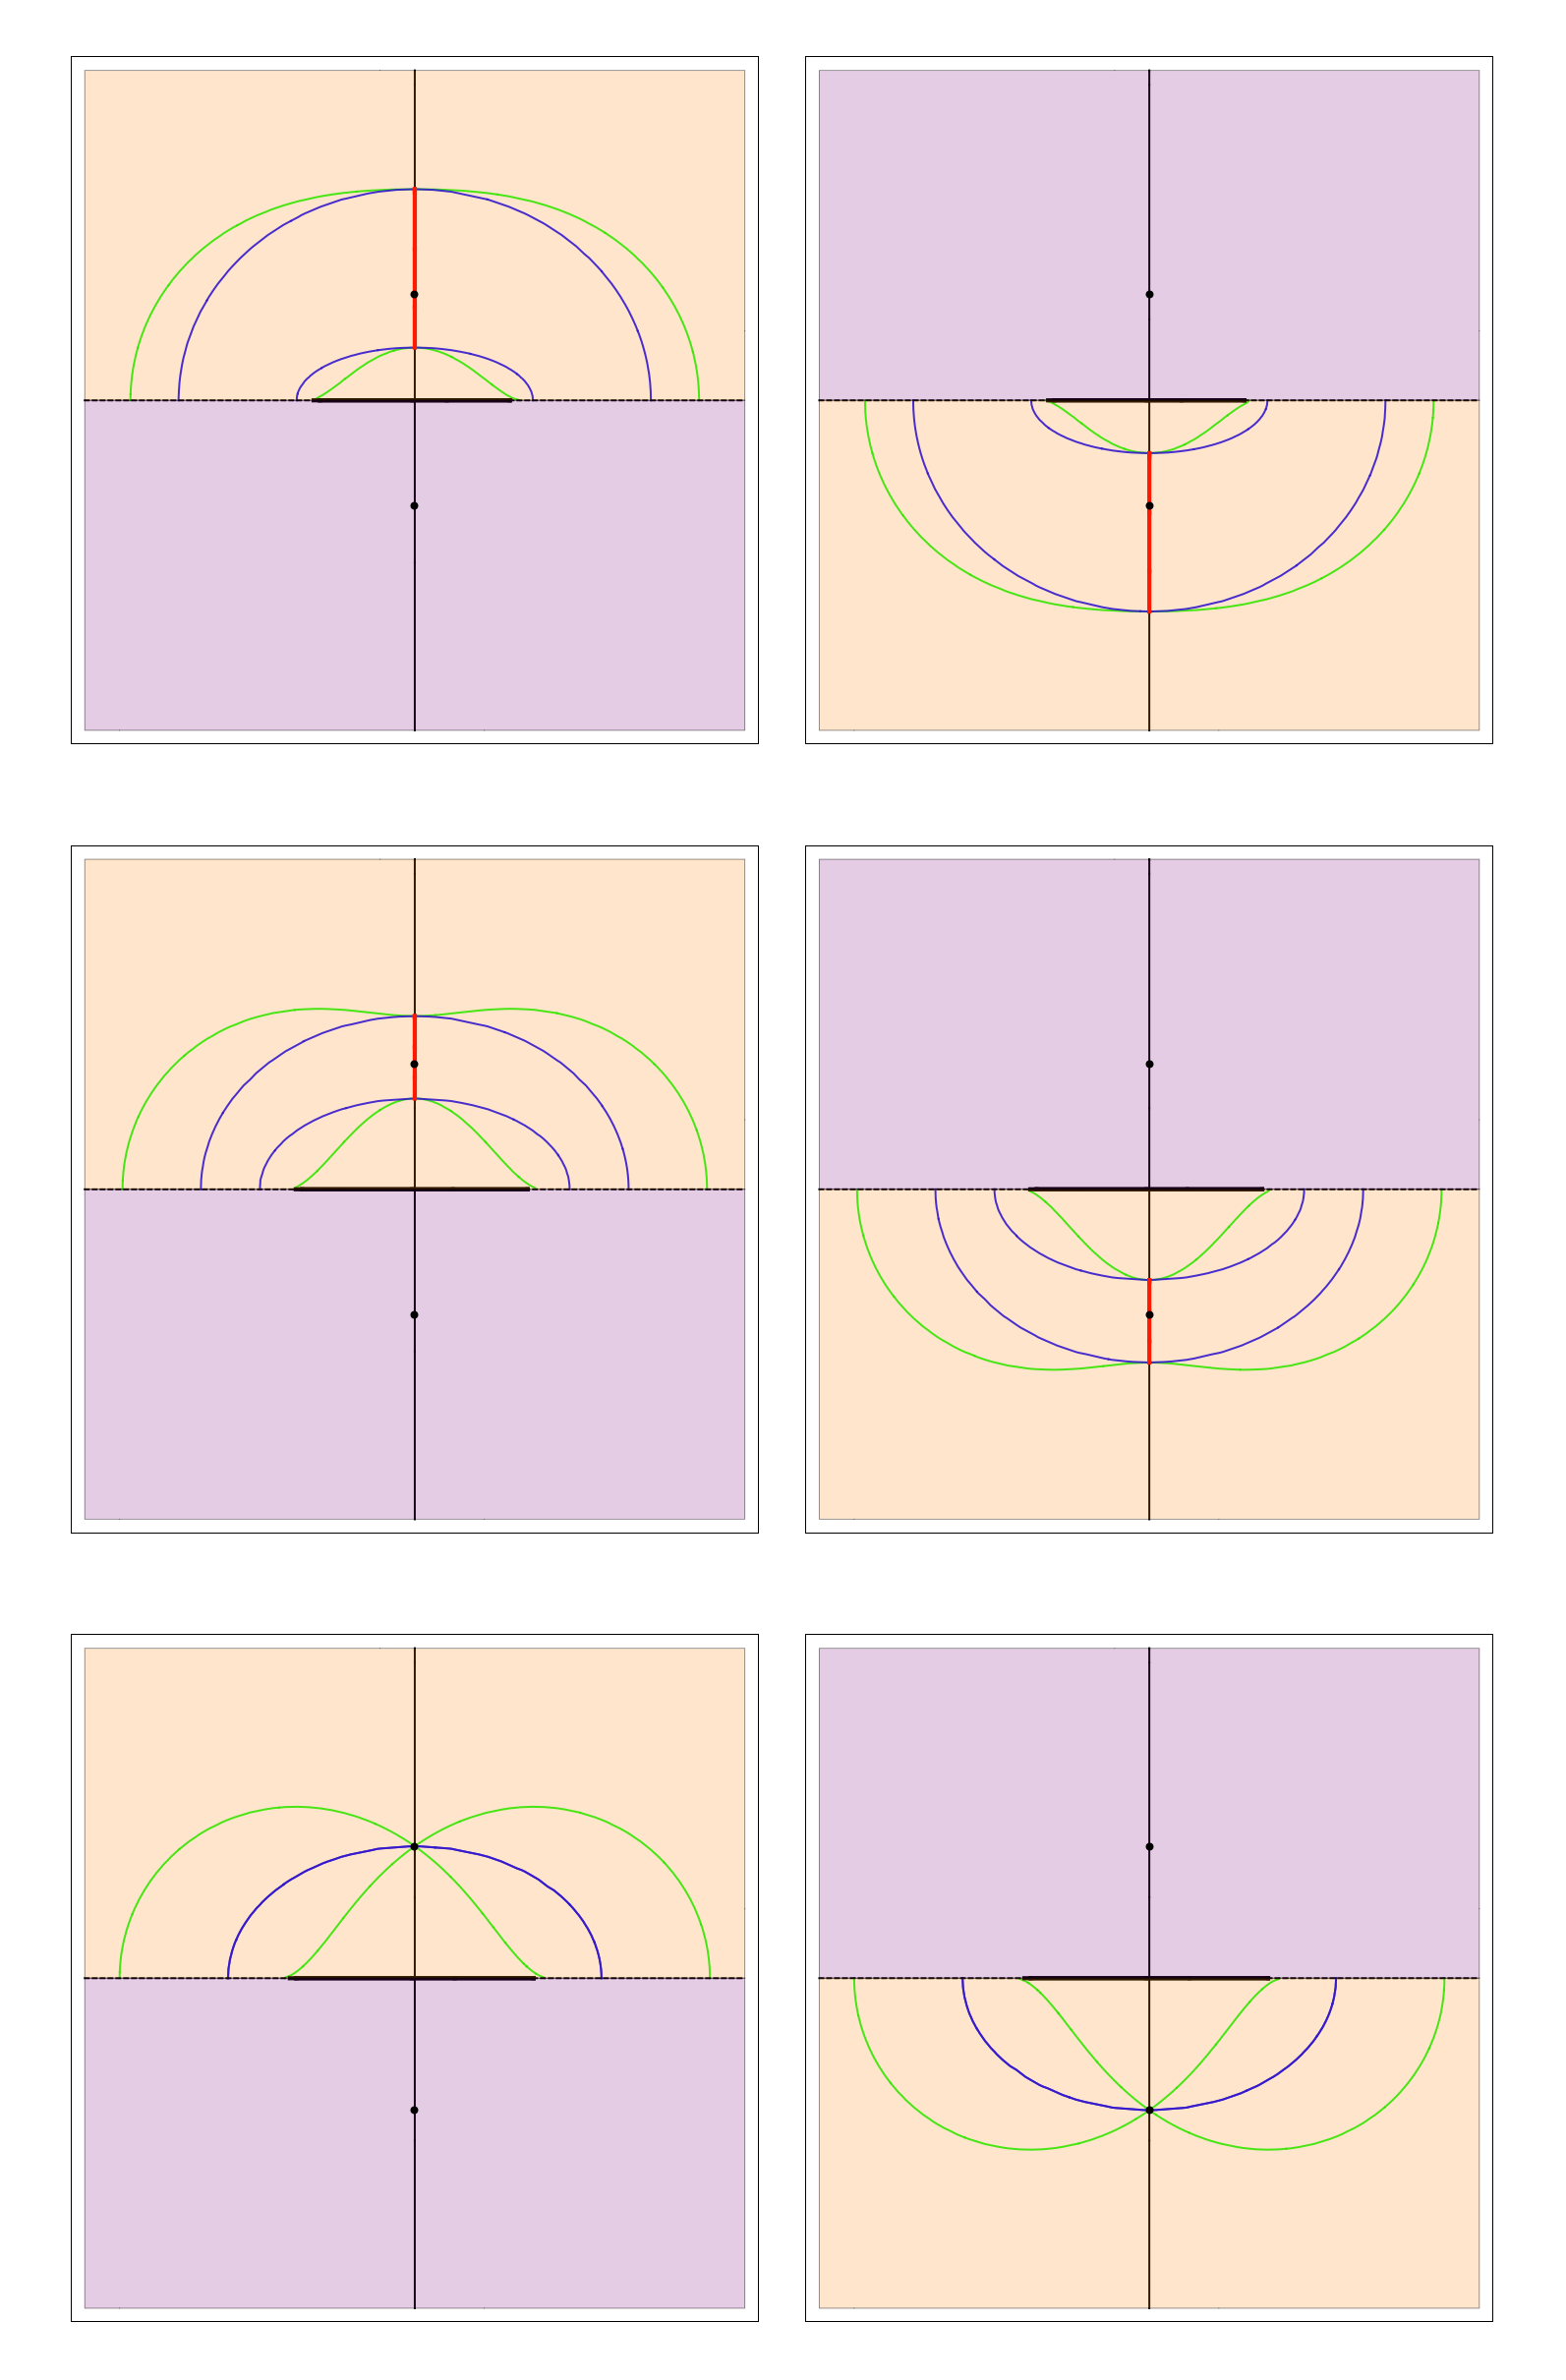
\includegraphics[width=0.85\textwidth]{img/Chapter3/Axis.png}}
 \end{center}
 \caption{Side view of the Kerr spacetime. The left column corresponds to $\mathcal{Z}_1$ and the right column for $\mathcal{Z}_2$. The yellow areas represent $\mathbb{R}_+$ and the pink ones represent $\mathbb{R}_-$. The green surfaces are the outer and inner ergospheres and the blue one are the outer and inner horizon. The red thick lines are the excluded regions in the $z$-axis and the black dots are the fixed points of the dynamic system. Notice that the inner and outer horizon coincide with the inner and outer ergosphere for the $z$-axis and all them collapse for $a=0$. The thick black line is the singular ring. Notice that as  $\mathbb{R}_-$ has no horizons, the pink regions has no curves, only the critical point at $\bar{z}=-a$. $M=1$ is settled for simplicity. }
 \label{fig:Axissurfaces}
\end{figure}  
As we can see in the phase portraits of \cref{fig:Phasediagrams,fig:Axissurfaces} the region $\bar z <0$ that corresponds on both cases to $\mathbb{R}_-$ has some kind of repulsive behavior. Indeed, the critical points in this region are always unstable saddle points, that behaves ''repelling`` the geodesic flow. Consider for example a geodesic that start in $\bar z_0 = -\infty$ with $\bar z_0'>0$. This geodesic will try to approach $\mathbb{R}_+$ but if the value of $\bar z_0'$ is not enough, the geodesic will be repealed by the singular point in $\bar z=-a$ and will end in $\bar z =-\infty$ again. If the geodesic has enough energy (enough value of $\bar z_0'$) it will defeat the repulsive behavior of the critical point at $\bar z=-a$  and it will end in $\mathbb{R}_+$ at $\bar z=\infty$. The minimum value of $\bar z'_0$ that allows a geodesic to travel from $\mathbb{R}_-$ to $\mathbb{R}_+$ is
\begin{equation}
 p_{\bar{z}_\text{critic}}^2-\frac{2 M \bar z_0}{a^2+\bar z_0^2}=\epsilon(p_{\bar{z}}=0,\bar{z}=-a) \quad \Longrightarrow \quad p_{\bar{z}_\text{critic}} =\bar z'_\text{critic}=\pm \frac{\sqrt{M} (a+\bar z_0)}{\sqrt{a} \sqrt{a^2+\bar{z}_0^2}}
\end{equation}
where $\bar{z}_0=\bar{z}(0)$. Note that $\epsilon(p_{\bar{z}}=0,\bar{z}=-a)=\frac{M}{a} $ which is the fraction of ''maximality'' of the black hole (remember that the black hole is said to be extremal when $M^2=a^2$).This can be visualize much more clearly in \cref{fig:zcritic} where we can easily realize that the geodesics with $\bar{z}'_0<\bar{z}'_\text{critic}$ does not have enough energy to get over the potential barrier and only the geodesies with $|\bar{z}'_0| \geq |\bar{z}'_\text{critic}|$ can pass through.
 \begin{figure}[hpt!] 
\begin{center}
 \centerline{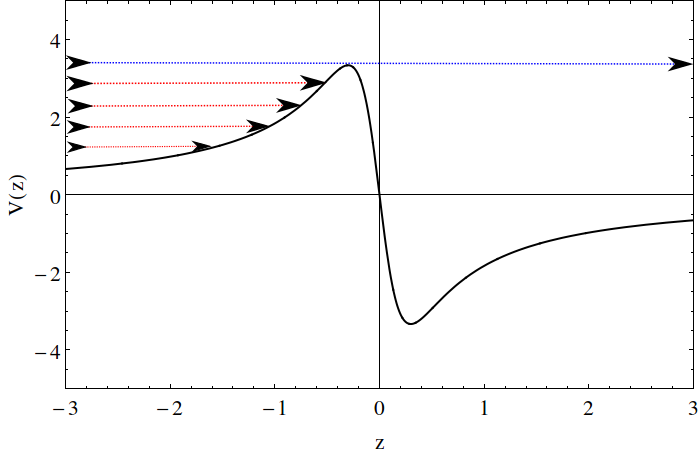
\includegraphics[width=0.7\textwidth]{img/Chapter3/Return.png}}
 \end{center}
 \caption{Potential $V(\bar z)$ and some trajectories that try to go from $\mathbb{R_-}$ to $\mathbb{R_+}$. The red trajectories correspond to values of $|z'_0|<|z'_\text{critic}|$ and the blue trajectory correspond to values of $z'_0=z'_\text{critic}$. $M=1$ is settled for simplicity.}
 \label{fig:zcritic}
\end{figure}  
In the space $\mathbb{R_+}$ the situation is the same, i.e. only geodesics with $|\bar{z}'_0|>|\bar{z}'_\text{critic}|$ will reach $\mathbb{R_-}$. Geodesics with a lower value of $|\bar{z}'_0|$ can oscillate around the critical point at $\bar{z}=a$ or reach a return point at end in $\bar z=\infty$. The geodesics that will reach a return point satisfies that
\begin{equation}
 \epsilon(p_{\bar{z}}=0,\bar{z}=-a)>\epsilon(p_{\bar{z}_0},\bar{z}_0)\geq 0 \quad \Longrightarrow  -|z'_\text{critic}|< p_{\bar{z}_0} =\bar{z}'_0 \leq - \frac{\sqrt{2 M \bar{z}_0} }{\sqrt{a^2+\bar{z}_0^2}}
\end{equation}
where $\bar{z}_0=\bar{z}(0)$. The return point is given by
\begin{equation}
 -\frac{2 M \bar{z}_\text{return}}{a^2+\bar{z}_\text{return}^2}=\epsilon(p_{\bar{z}_0},\bar{z}_0) \quad \Longrightarrow \quad \bar{z}_\text{return}=\frac{\sqrt{M^2-a^2 \left(p_{\bar{z}_0}^2-\frac{2 M \bar{z}_0}{a^2+z^2}\right)^2}-M}{p_{\bar{z}_0}^2-\frac{2 M \bar{z}_0}{a^2+z^2}}
\end{equation}
where $\frac{\sqrt{2 M \bar{z}_0} }{\sqrt{a^2+\bar{z}_0^2}}<|p_{\bar{z}_0}|<|p_{\bar{z}_\text{critic}}|$ and $\bar z>0$. Therefore values of $|p_{\bar{z}_0}|<\frac{\sqrt{2 M \bar{z}_0} }{\sqrt{a^2+\bar{z}_0^2}}$ with $\bar z>0$ correspond to geodesic that oscillate around $\bar z=a$. As we have commented before, this geodesic are traveling upwards in the \gls{PC} diagram changing from one patch to another.
 \begin{figure}[hpt!] 
\begin{center}
 \centerline{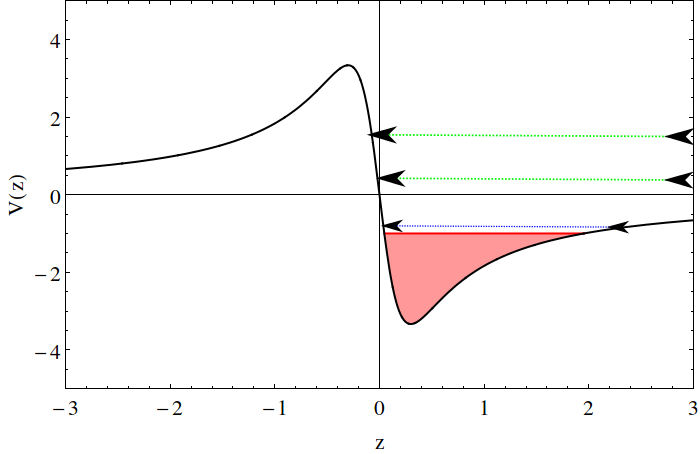
\includegraphics[width=0.7\textwidth]{img/Chapter3/Return2.png}}
 \end{center}
 \caption{Potential $V(\bar z)$ and some trajectories that try to go from $\mathbb{R_+}$ to $\mathbb{R_-}$ but does not reach the top of the potential. The green trajectories correspond to geodesics that end in $\bar z=\infty$ and the blue trajectory correspond to geodesics that oscillate around $\bar z=a$. The red region represents the excluded region, where no timelike particles are allowed. $M=1$ is settled for simplicity.}
 \label{fig:return2}
\end{figure} 
The return points of the oscillating movement given $\bar{z}_0=\bar{z}(0)$ and $p_{\bar{z}_0}=\bar p_z(0)$ are given by
\begin{equation}
  \bar{z}_{\text{return} \pm} =\frac{-M\pm \sqrt{M^2-a^2 \left(p_{\bar{z}_0}^2-\frac{2 M \bar{z}_0}{a^2+\bar{z}_0^2}\right)^2}}{p_{\bar{z}_0}^2-\frac{2 M \bar{z}_0}{a^2+\bar{z}_0^2}}
\end{equation}
where $|p_{\bar{z}_0}|<\frac{\sqrt{2 M \bar{z}_0} }{\sqrt{a^2+\bar{z}_0^2}}$ and $\bar z>0$.

\subsubsection{The \gls{SW} limit}

The \gls{SW} limit of the dynamic system correspond when $a\to 0$. In this limit the potential becomes $V(\bar z)=\frac{1}{\bar z}$, which coincide with the potential for a timelike test particle moving with $L=0$ (where $L$ is the angular momentum) in the \gls{SW} geometry (see \cite{hawking1973large}). This potential also coincide with the Newtonian motion of a test particle moving in radial trajectories as the \gls{SW} potential for timelike test particles coincide with the Newtonian potential iff $L=0$. But in this case more information is provided by the dynamical system. Only the region $\mathbb{R}_+$ coincide with the radial movement for timelike particles in the \gls{SW} geometry, while the movement in the $\mathbb{R}_-$ space coincide with the radial geodesics in the \gls{SW} geometry with negative mass. As we can see in the phase portrait of the \cref{fig:alimit}, the two regions $\mathbb{R}_-$ and $\mathbb{R}_+$ are now disconnected and no geodesic can go from one to another. This is the only case in which this disconnection of the regions $\mathbb{R}_-$ and $\mathbb{R}_+$ occurs. This fact can be understand as the ring singularity  became a single point because the singular ring collapses and the inner disk with it, leaving the two cited regions disconnected. Now, the two $z$-axis of the Kerr geometry exist separately in the sense that for each axis, now the part with $\bar z>0$ and $\bar z<0$ is in the same spacetime (remember that the existence of the inner disk separate the \gls{MAE} in the regions $\mathcal{Z}_1$ and $\mathcal{Z}_2$). 
 \begin{figure}[b!] 
\begin{center}
 \centerline{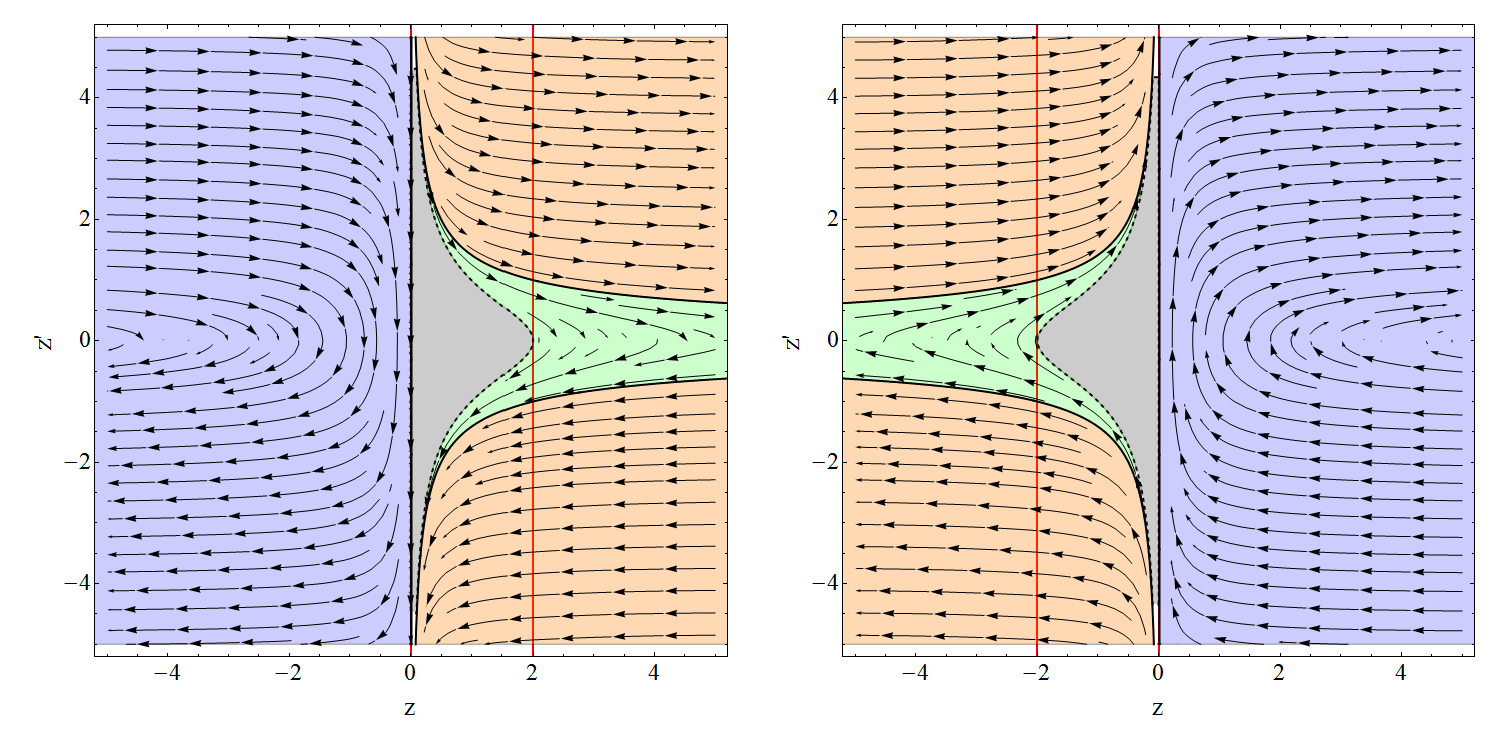
\includegraphics[width=\textwidth]{img/Chapter3/lim.png}}
 \end{center}
 \caption{Schwarzschild limit of the dynamic system. The red lines corresponds to the horizons at $\bar z=2M$. The red region corresponds to the excluded region, the blue area represent the curves that start in $\bar z=-\infty$ and return to $\bar z=-\infty$, the orange zones represent the curves that start in $\bar z=\infty$ and end in $\bar z=\infty$. The closed curves are in the green area and the limit orbit is the black dashed line surrounding the excluded region. $M=1$ is settled for simplicity.}
 \label{fig:alimit}
\end{figure}  
The fact that $\mathbb{R}_-$ (which corresponds to the space where $r(x,y,z)<0$) has a repulsive behavior leads in the fact that the Kerr metric has an isometry given by
\begin{align}
 M &\to - M\\
 r &\to - r
\end{align}
being checked more easily when the metric is in \gls{BL} coordinates (see \cref{eq:Kerrmetricblsimpl}). The \gls{SW} limit has geodesics that can reach the asymptotically flat region at $\bar z=\infty$ and geodesics that get trapped by the black hole. The escape velocity is easily computed as
\begin{equation}
 \frac{1}{\bar{z}_0}+p_{\bar{z}_0}^2=0 \quad \Longrightarrow \quad p_{\bar{z}_0} = \pm \frac{\sqrt{2 M}}{\sqrt{\bar z}}.
\end{equation}
Notice that in the horizon $\bar z=2M$ the escape velocity is $p_{\bar{z}_0}=\bar{z}'_0= \pm 1$, which in regular units correspond to $\bar{z}'_0=c$, where $c$ is the speed of light. For points $\bar z<2M$ the escape velocity is $\bar{z}'_0>c$ and no timelike particles can escape. Obviously, this is in perfect match with the results given in \cref{causalstruct}, where we obtained that once crossed $\bar z=r_+=2M$ (for $a=0$) no timelike particle can go back, and as now $\bar z=r_-=0$ (which coincides with the singularity) the particle cannot change to another \gls{KS} patch because it will fall into the singularity.

\subsubsection{Oscillation frequencies in extreme Kerr}
\FloatBarrier
We have seen that the existence of the excluded regions is translated in the fact that no timelike particles can be in the stable point at $\bar z=a$. But as we have studied in \cref{excludedreg}, the excluded regions for $a=M$ vanishes. However, as we also saw in \cref{excludedreg}, only null geodesic can remain in this critical point, but timelike particles are able to oscillate around this point. In the extreme Kerr ($a=M$) we can linearize the potential $V(\bar z)$ around the critical point in order to obtain the oscillating frequency.
 \begin{figure}[b!]
\begin{center}
 \centerline{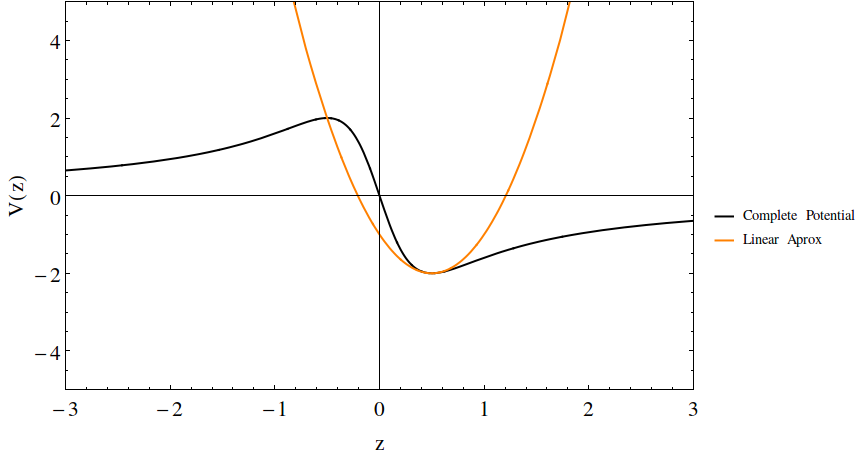
\includegraphics[width=\textwidth]{img/Chapter3/Lineal.png}}
 \end{center}
 \caption{Linearizion of the potential $V(\bar z)$ around the critical point at $\bar z =a$. The black line represent the complete potential and the green line correspond to the second order linearization, which transforms the problem into a harmonic oscillator.}
 \label{fig:2}
\end{figure}  
We can linearize the potential to its second order as (remember that we can only do this for the extreme Kerr in which $a=M$)
\begin{equation}
 V( \bar z) - V(a=M)=\frac{ (z-M)^2}{2 M^2} +O(\bar z-M)^3  
\end{equation}
The linealization of the potential can be visualized in \cref{fig:2}. The dynamic equations are
\begin{align}
 \bar{z}'(s)&=p_{\bar{z}}, \\
 p_{\bar{z}}'(s)&=- \partial_{\bar{z}} V(\bar{z})=-\frac{(z-M)}{M^2}.
\end{align}
The solution to this system with initial values $\bar z(0)=\bar{z}_0$ and $p_{\bar{z}}(0)=p_{\bar{z_0}}$ is
\begin{align}
 \bar z(s)&=p_{\bar{z_0}} \cos \left(\frac{s}{M}\right)+\frac{(M-\bar{z}_0) \sin \left(\frac{s}{M}\right)}{M},\\
 p_{\bar{z}}(s)&= M p_{\bar{z_0}} \sin \left(\frac{s}{M}\right)+(\bar{z}_0-M) \cos \left(\frac{s}{M}\right)+M.
\end{align}
The oscillating frequency is
\begin{equation}
 \nu=\frac{1}{M}.
\end{equation}
We conclude that when the Kerr black hole is more massive the particle oscillate slower. This is quite surprising because a greater value of the mass of the black hole acts ''bounding`` the particle to $\bar z=a=M$.

\subsubsection{Stability of the critical point}

We are now interested in the Stability of the $z$-axis itself. This is because unless we have seen that there exist critical points in the axis, we want to know what would happen to this critical points if a little perturbation in every direction is done. This can have two possible consequences, that the particle return to the $z$-axis or go away. This will give us useful information about if the symmetry axis is stable or unstable. To analyze this we will need the full Hamiltonian to perform the perturbation. The Kerr metric in \gls{KS} coordinates is
\begin{equation}\label{eq:KSmetriclin}
 g=\eta + h K \otimes K,
\end{equation}
where $\eta$ is the Minkowsky metric and
\begin{align}
 f&=\frac{2 M r^3}{r^4+a^2 z^2}, \nonumber \\
 K&=-\sigma dt + \frac{r(x dx+y dy)}{r^2+a^2} + \frac{a(x dy-y dx)}{r^2+a^2}+\frac{z dz}{r}. \nonumber
\end{align}
We have now to repeat all the steps that we performed on \cref{Hamiltonianbon} to obtain a full Hamiltonian to the general Kerr geodesic. As we use before, affinely parametrized geodesics are the solutions of the Hamilton equations of the Hamiltonian
\begin{equation}
H=\frac{1}{2}(g^{-1})^{\alpha \beta} p_\alpha p_\beta
\end{equation}
defined on the cotangent bundle of $\M$. the Hamilton equations fix $\bm{p}= g (u, \cdot)$ where $u$ is  the tangent vector to the geodesic. Using  the explicit expression (\ref{eq:KSmetriclin}) for the metric, this Hamiltonian takes the form
\begin{equation}
H= \frac{1}{2} \left(
\eta^{\alpha \beta} p_\alpha p_\beta -  h (K^\alpha p_\alpha)^2
\right).
\end{equation}
Given that $\partial_t$ is a Killing vector,the quantity $E := - \bm{p} (\partial_t)$ is conserved along geodesics.
Note also that, with this definition,
\begin{equation}
K^{\alpha} p_{\alpha} = - E \Khat + \vec{K} \cdot \vec{p},
\end{equation}
where we have written $\bm{p} = \{ \phat,
\vec{p} \, \}$ and dot means scalar product with $\delta_{ij}$.

The Hamiltonian itself is a conserved quantity with the value of
$H=-\frac{1}{2} \mu$ where $\mu= {0,\pm 1}$ depending on whether the
geodesic is timelike ($\mu=1$), spacelike ($\mu=-1$) or null
($\mu=0$). Inserting (\ref{Kdotp}) and the conserved quantity $E$
into (\ref{Hamiltonkerrschild})
the following Hamiltonian arises naturally
\begin{equation}\label{FinalgeneralH}
H^{\prime} := H + \frac{1}{2} E^2 = 
\frac{1}{2} \left( \vec{p}^{\,2}- h \left( \vec{K} \cdot \vec{p} - E 
\Khat \right)^2 \right),
\end{equation} 
which is now defined on the cotangent 
bundle of $\mathbb{R}^{3} \setminus \C$, where $\C$ represent the singular ring. 

We will perform the perturbations for $\mathcal{Z}_1$ because the perturbations for $\mathcal{Z}_2$ have the same behavior but changing the sign of $z$. The point $z=-a$ result appropriate to analyze because timelike particles are allowed to be at rest for every value of $a$. Suppose that the particle is at rest in $z=a$. As a rest particle in the $z$ axis has $\dot{z}=0$, we can use \cref{Hameje1,Hameje2} to solve for $p_z$ in the rest point of $z=-a$ to get that $p_z(z=-a,\dot{z}=0)=\frac{E M}{a+M}$. As the particle start at rest in the rest of the variables $p_x=p_y=p_z=x=y=0$ are settled and then a perturbation is performed as
\begin{align}
 x & \to \delta x,\\
 y & \to \delta y,\\
 z & \to -a+ \delta z,\\
 p_x & \to \delta p_x,\\
 p_y & \to \delta p_y,\\
 p_z & \to \frac{E M}{a+M}+\delta p_z.\\
\end{align}
The Hamilton equations linearized at it first order in the Hamiltonian variables product of the perturbation $\{ \delta x,\delta y,\delta z, \delta p_x,\delta p_y,\delta p_z \}$ can be written as
\begin{equation}
 \vec{\xi}'(s)= \vec{\xi}_0 \delta E+\mathcal{A} \vec{\xi}(s)
\end{equation}
where $\vec{\xi}_0=\vec{\xi}_0(M,a)$ is a non-homogeneous term,the perturbation variables are collected in the vector $\vec{\xi}(s)=\{ \delta x(s),\delta y(s),\delta z(s), \delta p_x(s),\delta p_y(s),\delta p_z(s) \}$ and the matrix $\mathcal{A}$ is given by
\begin{equation}
\mathcal{A}=
\begin{mpmatrix}
 \frac{M E}{2 a^2+2 M a} & -\frac{M E}{2 a (a+M)} & 0 & 1 & 0 & 0 \\
 \frac{M E}{2 a^2+2 M a} & -\frac{M E}{2 a (a+M)} & 0 & 1 & 0 & 0 \\
 0 & 0 & 0 & 0 & 0 & \frac{a+M}{a} \\
 -\frac{M (a+2 M) E^2}{4 a^2 (a+M)^2} & 0 & 0 & -\frac{M E}{2 a (a+M)} & -\frac{M E}{2 a (a+M)} & 0 \\
 0 & -\frac{M (a+2 M) E^2}{4 a^2 (a+M)^2} & 0 & \frac{M E}{2 a^2+2 M a} & -\frac{M E}{2 a (a+M)} & 0 \\
 0 & 0 & \frac{M E^2}{2 a (a+M)^2} & 0 & 0 & 0 \\
\end{mpmatrix}.
\end{equation}
where $E=\frac{\sqrt{a+M}}{\sqrt{a}}$ is the energy of the rest particle at $z=-a$. The eigenvalues of this matrix are
\begin{equation}
\hspace{-0.15\textwidth}
\begin{aligned}
&\lambda_1=-\sqrt{\frac{M}{2 a^3}} \quad \quad \lambda_2=\sqrt{\frac{M}{2 a^3}} \quad \quad \lambda_3=-\frac{1}{2} i \sqrt{\frac{M \left(2 \left(\sqrt{M (a+M)}+M\right)+a\right)}{a^3 (a+M)}}\\
&\lambda_4=\frac{1}{2} i \sqrt{\frac{M \left(2 \left(\sqrt{M (a+M)}+M\right)+a\right)}{a^3 (a+M)}} \quad \lambda_5=-\frac{1}{2} i \sqrt{\frac{M \left(-2 \sqrt{M (a+M)}+a+2 M\right)}{a^3 (a+M)}}\\
&\hspace{0.3\textwidth} \lambda_6=\frac{1}{2} i \sqrt{\frac{M \left(-2 \sqrt{M (a+M)}+a+2 M\right)}{a^3 (a+M)}}
\end{aligned}.
\end{equation}


 \begin{figure}[ht!]
\begin{center}
 \centerline{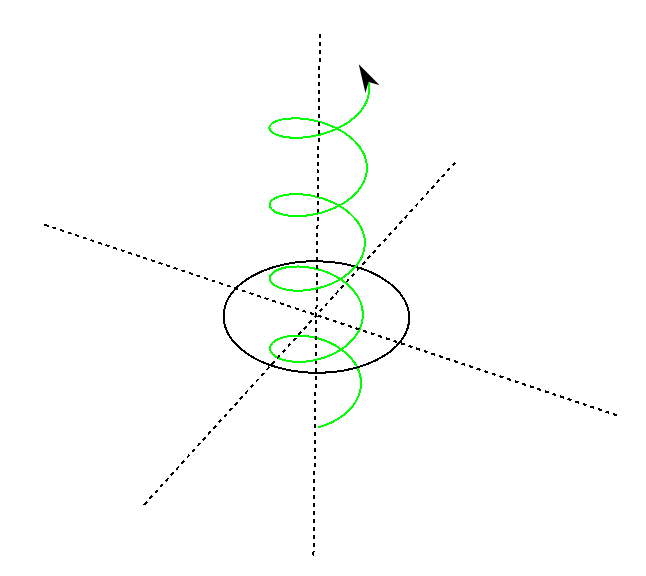
\includegraphics[width=0.75\textwidth]{img/Chapter3/lineje1.png}}
 \end{center}
 \caption{Representation of the movement at its first order after the perturbation in the unstable saddle point $z=-a$. In this image $\delta p_z>0$ and therefore, the geodesic moves upwards. The thick dashed lines represent the Cartesian axes, the green thick line is the geodesic movement and the black thick ring represents the singular ring.}
 \label{fig:spiral1}
\end{figure} 

The two first eigenvalues are associated with $z$ and $p_z$. This is more clear if we rewrite the matrix $\mathcal{A}$ in the base $\{ \delta x(s),\delta px(s),\delta y(s), \delta p_y(s),\delta z,\delta p_z(s) \}$ because in this base the matrix decompose in two Jordan boxes as
\begin{equation}
\mathcal{A}'=
\begin{mpmatrix}
 \frac{M E}{2 a^2+2 M a} & 1 & -\frac{M E}{2 a (a+M)} & 0 & 0 & 0 \\
 -\frac{M (a+2 M) E^2}{4 a^2 (a+M)^2} & -\frac{M E}{2 a (a+M)} & 0 & -\frac{M E}{2 a (a+M)} & 0 & 0 \\
 \frac{M E}{2 a^2+2 M a} & 0 & \frac{M E}{2 a^2+2 M a} & 1 & 0 & 0 \\
 0 & \frac{M E}{2 a^2+2 M a} & -\frac{M (a+2 M) E^2}{4 a^2 (a+M)^2} & -\frac{M E}{2 a (a+M)} & 0 & 0 \\
 0 & 0 & 0 & 0 & 0 & \frac{a+M}{a} \\
 0 & 0 & 0 & 0 & \frac{M E^2}{2 a (a+M)^2} & 0 \\
\end{mpmatrix}.
\end{equation}
and now it is clear that the eigenvalues of $z$ and $p_z$ are $\lambda_{\pm}=\pm \sqrt{\frac{M E^2}{2 a (a+M)^2} \frac{a+M}{a} }=\pm \sqrt{\frac{M}{2 a^3}}$. As $M>a$ the eigenvalues $\lambda_3$,$\lambda_4$,$\lambda_5$,$\lambda_6$ are purely imaginary and therefore the point $z=-a$ happens to be a saddle point along the $z$ axis (as we already know) and a center along the $\{x,y\}$ plane. So if a perturbation that takes away the geodesic from the axis is performed, the particle oscillates around $z=-a$ unless $\delta p_z \neq 0$, in which case the particle moves spirally along the z axis upwards if $\delta p_z>0$ and downwards if $\delta p_z<0$. This is of course the composition of the movement in the $z$ axis with a center-like movement in the $\{x,y\}$ plane. The real movement (not only the first order) of the perturbed geodesic can be found through numerical integration in the last image of the \cref{ch:nsog}.

Now that we know the behavior of the unstable point at $z=-a$ we we could think of analyzing the stable point at $z=a$ but as we prevent previously, this point is not allowed to timelike particles because of the excluded region. Even when $a \to M$, the point is still inaccessible to timelike particles as we saw in \cref{causalstruct}. Either way, the stability behavior of the whole axis is expected to be the same as when we linearize the Hamiltonian equations around an arbitrary value of $z_0$ and $p_{z_0}$ the matrix that we obtain already have the same structure as the one that we obtain when we linearize the axis, but with much more complicated terms that are not very enlightening to display here. 
\FloatBarrier
\section{Lower energy orbit}
 \begin{figure}[b!]
\begin{center}
 \centerline{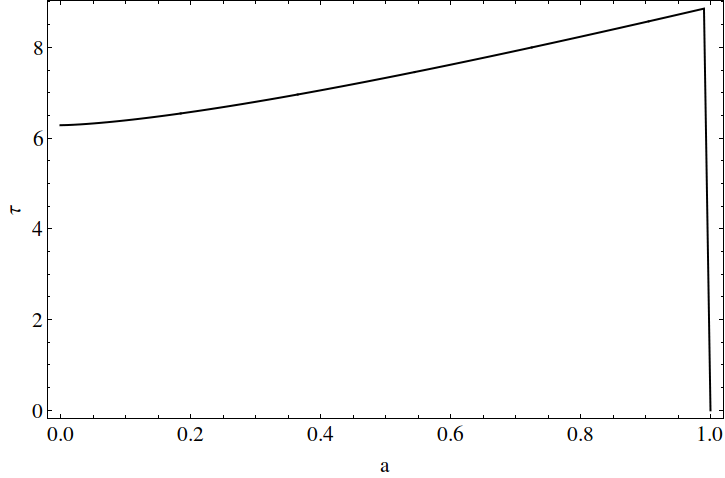
\includegraphics[width=0.85\textwidth]{img/Chapter3/travel.png}}
 \end{center}
 \caption{Period of the lower energy orbit as a function of the parameter $a$. For simplicity $M=1$ is chosen.}
 \label{fig:travel}
\end{figure}  
We are now interested in the lower energy orbit. As we notice in \cref{excludedreg} this orbits are the boundary of the excluded regions and the last orbit that is allowed as we approach the forbidden region. We can compute the propper time ($\tau$) that this geodesic (that as we have seen before, is a closed curve in the phase portrait and therefore corresponds to a periodic orbit) needs to complete a full turn around the forbidden region. Also, we know that the forbidden region for every value of the parameter $a$ is always between in the interval $[r_-,r_+]$. To compute the period of this movement we must use the energy equation. In virtue of \cref{epsilonrange} we know that the lower energy orbit satisfies
\begin{equation}
 (z')^2-\frac{2 M z}{a^2+z^2}=2 \epsilon=-1.
\end{equation}
 \begin{figure}[hpt!]
\begin{center}
 \centerline{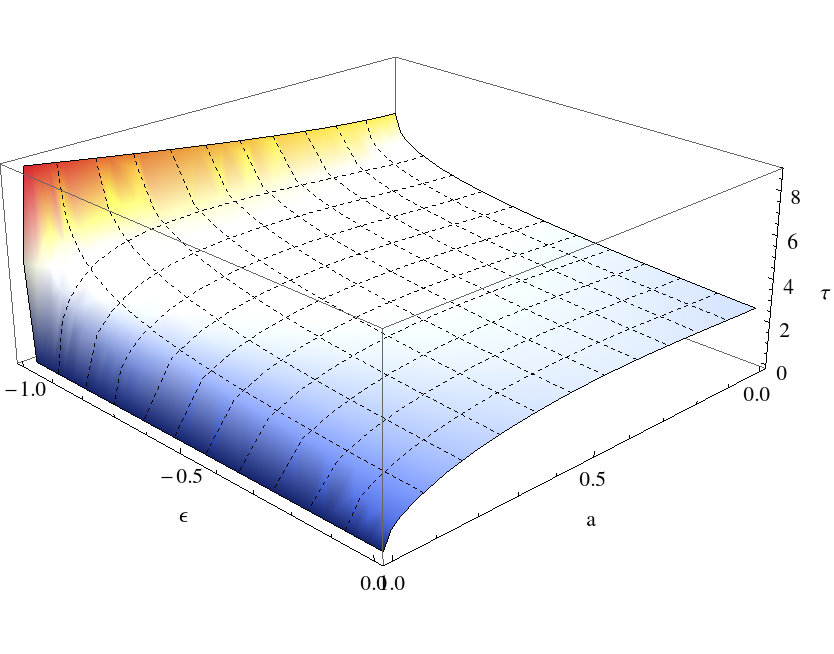
\includegraphics[width=0.85\textwidth]{img/Chapter3/travel2.png}}
 \end{center}
 \caption{Period of the bounded orbit as a function of the parameter $a$ and the Newtonian energy $\epsilon$. For simplicity $M=1$ is chosen.}
 \label{fig:travelother}
\end{figure} 
We can now solve for $z'$ as
\begin{equation}
 z'= \pm \frac{\sqrt{z (2 M-z)-a^2}}{\sqrt{a^2+z^2}}.
\end{equation}
Using this relation we can write
\begin{equation}
 \int_0^T dt = \int_{r_-}^{r_+} \frac{1}{\frac{\sqrt{2 M z-\left(a^2+z^2\right)}}{\sqrt{a^2+z^2}}} dz
\end{equation}
This integral has a very complicated expression for a general value of $a\in[0,M]$ that can be visualized in \cref{fig:travel}, but for $a=0$ we can compute this integral analytically as
\begin{equation}
\begin{aligned}
&2\int_{0}^{2M} \frac{z}{\sqrt{z (2 M-z)}} dz = \nonumber \\
& \left. -2\left( \sqrt{z (2 M-z)} \left(\frac{2 M \log \left(\sqrt{z-2 M}+\sqrt{z}\right)}{ \sqrt{z^2-2 M z}}+1\right) \right) \right|_{0}^{2M} = 2\pi M
 \end{aligned}
\end{equation}
which coincides with two times the maximum time of a timelike particle to fall from the even horizon into the singularity in the \gls{SW} geometry. Notice that this period is the maximum time that a timelike geodesic expends traveling from $r_-$ to $r_+$. This can be checked analyzing the behavior of the bounded orbits ($\epsilon \in [-\frac{1}{2},0]$) as is displayed in \cref{fig:travelother}. In this figure we can see that the travel time is always $\tau<\tau(\epsilon=-\frac{1}{2})$.

This analysis reveal interesting features. First of all, notice that the time for $a=1$ is $\tau=0$ because in this limit $r_-=r_+$. But what is really unexpected is the fact that the period of the lower energy orbit is greater as the parameter $a$ increases. This is very strange because the area of the excluded regions decreases as the parameter $a$ increases as we saw in \cref{excludedreg}, and therefore the boundary of the excluded regions (which is the lower energy orbit) decreases as well.